% --------------------------------------------------
% Capítulo 2: Posicionamento de EDUs
% --------------------------------------------------
\chapter{On the Positioning of Emergencies Detection Units Based on Geospatial Data of Urban Response Centres}
\label{cap:posicionamento}

\begin{refsection}

\textbf{ABSTRACT}

Urban areas have been subject to emergency situations with different causes and sometimes dramatic consequences. With the advent of smart cities technologies, multi-emergency detection units could be conceived and implemented taking advantage of affordable sensing technologies and efficient decision algorithms, allowing quick and distributed detection of emergencies. However, a recurrent problem has been the positioning and further deployment of such detection units in a way that the particularities of each target city are properly considered. In this sense, this article proposes the processing of geospatial data about existing urban infrastructure associated with some critical response after an emergency is detected, selecting hospitals, police stations, fire departments, and metro stations, in the target city. These infrastructures are then exploited to define the novel concept of mitigation zones, which indirectly express the perceived level of urban resilience to emergencies. Then, four positioning algorithms are proposed to exploit the mitigation zones considering a defined set of available detection units for deployment. Since the proposed approach is valid for any city, provided that geospatial data is available, it could be largely adopted to support different smart city systems, potentially bringing significant results in this area.

\textbf{Keywords:} Smart cities, Sustainable and resilient cities, Emergency detection, Sensors positioning, Urban infrastructure.

\section{Introduction}
\label{c2:introduction}

The development of more sustainable and resilient cities has been a major goal when the intense urbanisation process and the climatic changes are posed as dramatic challenges of our times \cite{surveycity3}. Lately, with the advent of new hardware, software, and communication technologies to support the development of more comprehensive cyber-physical systems \cite{surveycityPlatform1,surveycityPlatform2,surveycityPlatform3}, smart cities initiatives have emerged to bring innovative solutions to such complex challenges. In this context, some systems that are conceived to detect one or more types of urban emergencies and to act properly have gained attention, opening a new age for emergency and disaster management \cite{surveyEmergencies}. 

Any number and types of sensors can be attached to a Single-Board Computer (SBC) or a Microcontroller Unit (MCU) to create a multi-sensor Emergencies Detection Unit (EDU), which will be connected to some wired or wireless network to report when one or more critical situations are detected. The EDUs may be programmed to process data locally, defining on-the-edge approaches when detecting emergencies \cite{smartcitiesedge}, or they can rely on cloud-based architectures to distributively process data \cite{smarticiteshibrid}. Whatever the case, for a defined set of available EDUs to be deployed, a complex issue has been to find the best positions for them, which may consider not only technological issues but also the geospatial configurations of a city. Furthermore, since some positioning solutions have been tailored to specifically fit within the constraints of a particular city \cite{positions1,positions2}, a solution to this positioning challenge should also be adaptable enough to be efficiently applied to any city in the world. 

The problem of positioning sensor-based units has been usually approached by the understanding of the target city \cite{spatial2}. Generally speaking, a city is a very complex scenario comprised of people, its environment and existing infrastructure, which impact the way we live in urban areas. When taking the problem of emergencies management, comprising its detection, alerting and mitigation, the people-environment-infrastructure elements are highly related, intrinsically affecting each other. Particularly, the existing infrastructure associated with emergency mitigation, which is related to the actions taken after an emergency of any type is detected, can be leveraged as an important information when assessing the level of resilience of any city, potentially saving lives. As any emergency is being addressed following this concept, for any environmental adverse conditions, a comprehensive perception of urban emergency response is achieved. This multi-perspective reasoning can directly guide the deployment of EDUs for any city, in a more adaptive way, potentially improving the overall detection efficiency of the employed system.

For the EDUs positioning problem based on mitigation response centres in the form of existing urban infrastructure, we use geospatial data as the main reference when defining the proposed concept of Mitigation Zones (MZ). A MZ is defined based on the principle that when an emergency occurs, the city will try to act on that emergency in some way, either trying to cease the causes of the emergency or performing rescue and medical assistance operations for affected people. For example, mitigation actions may be associated with calling ambulances, dispatching fire trucks or diverting traffic flows. These actions, commonly referred as ``emergency mitigation'', may be performed by any emergency management system and the literature has presented many solutions for that \cite{surveyEmergencies,mitigation1,mitigation2}. The association of response centres with Mitigation Zones is the core element when guiding the positioning of EDUs in this article.

A mitigation response centre is defined as a Point of Interest (PoI), with hospitals, fire departments, police stations/posts, and metro stations (a type of urban mobility hub) as the list of PoIs to be considered. During an emergency, it is reasonable to expect that the distance between the affected area (emergency's spot) and the active set of PoIs in a city will be crucial when performing mitigation actions, since areas farther from response centres will be harder to be supported during an emergency, on average. This way, Mitigation Zones will be created according to the normalised distances to all PoIs in a city, automatically, according to a defined mathematical model. As the list of PoIs can be directly retrieved from open databases as OpenStreetMap, any city can be divided into multiple Mitigation Zones, making the proposed solution more flexible.

%%%
Four algorithms will be proposed to indicate the positions of the EDUs: Random, Balanced, Balanced+ and Restricted. For all proposed algorithms, it is considered the severity index of the zones as an input parameter, with a higher severity level zone (worse served by response centres concerning the computed normalised distances) proportionally receiving more EDUs than other mitigation zones closer to the considered list of PoIs. With that, a suggested position for each EDU can be achieved, which will further support the actual physical deployment of the nodes in a city. All proposed algorithms will be implemented and evaluated for the cities of Porto (Portugal) and Paris (France), with real data for the PoIs being considered. 

Figure \ref{fig:smartcity} presents a conceptual representation of how mitigation zones can be exploited to support the positioning of sensor nodes. The idea is that mitigation zones may be processed as data layers, each one comprising a particular perception of a target area according to the desired level of details being modelled.

\begin{figure}[htbp!]
    \centering
    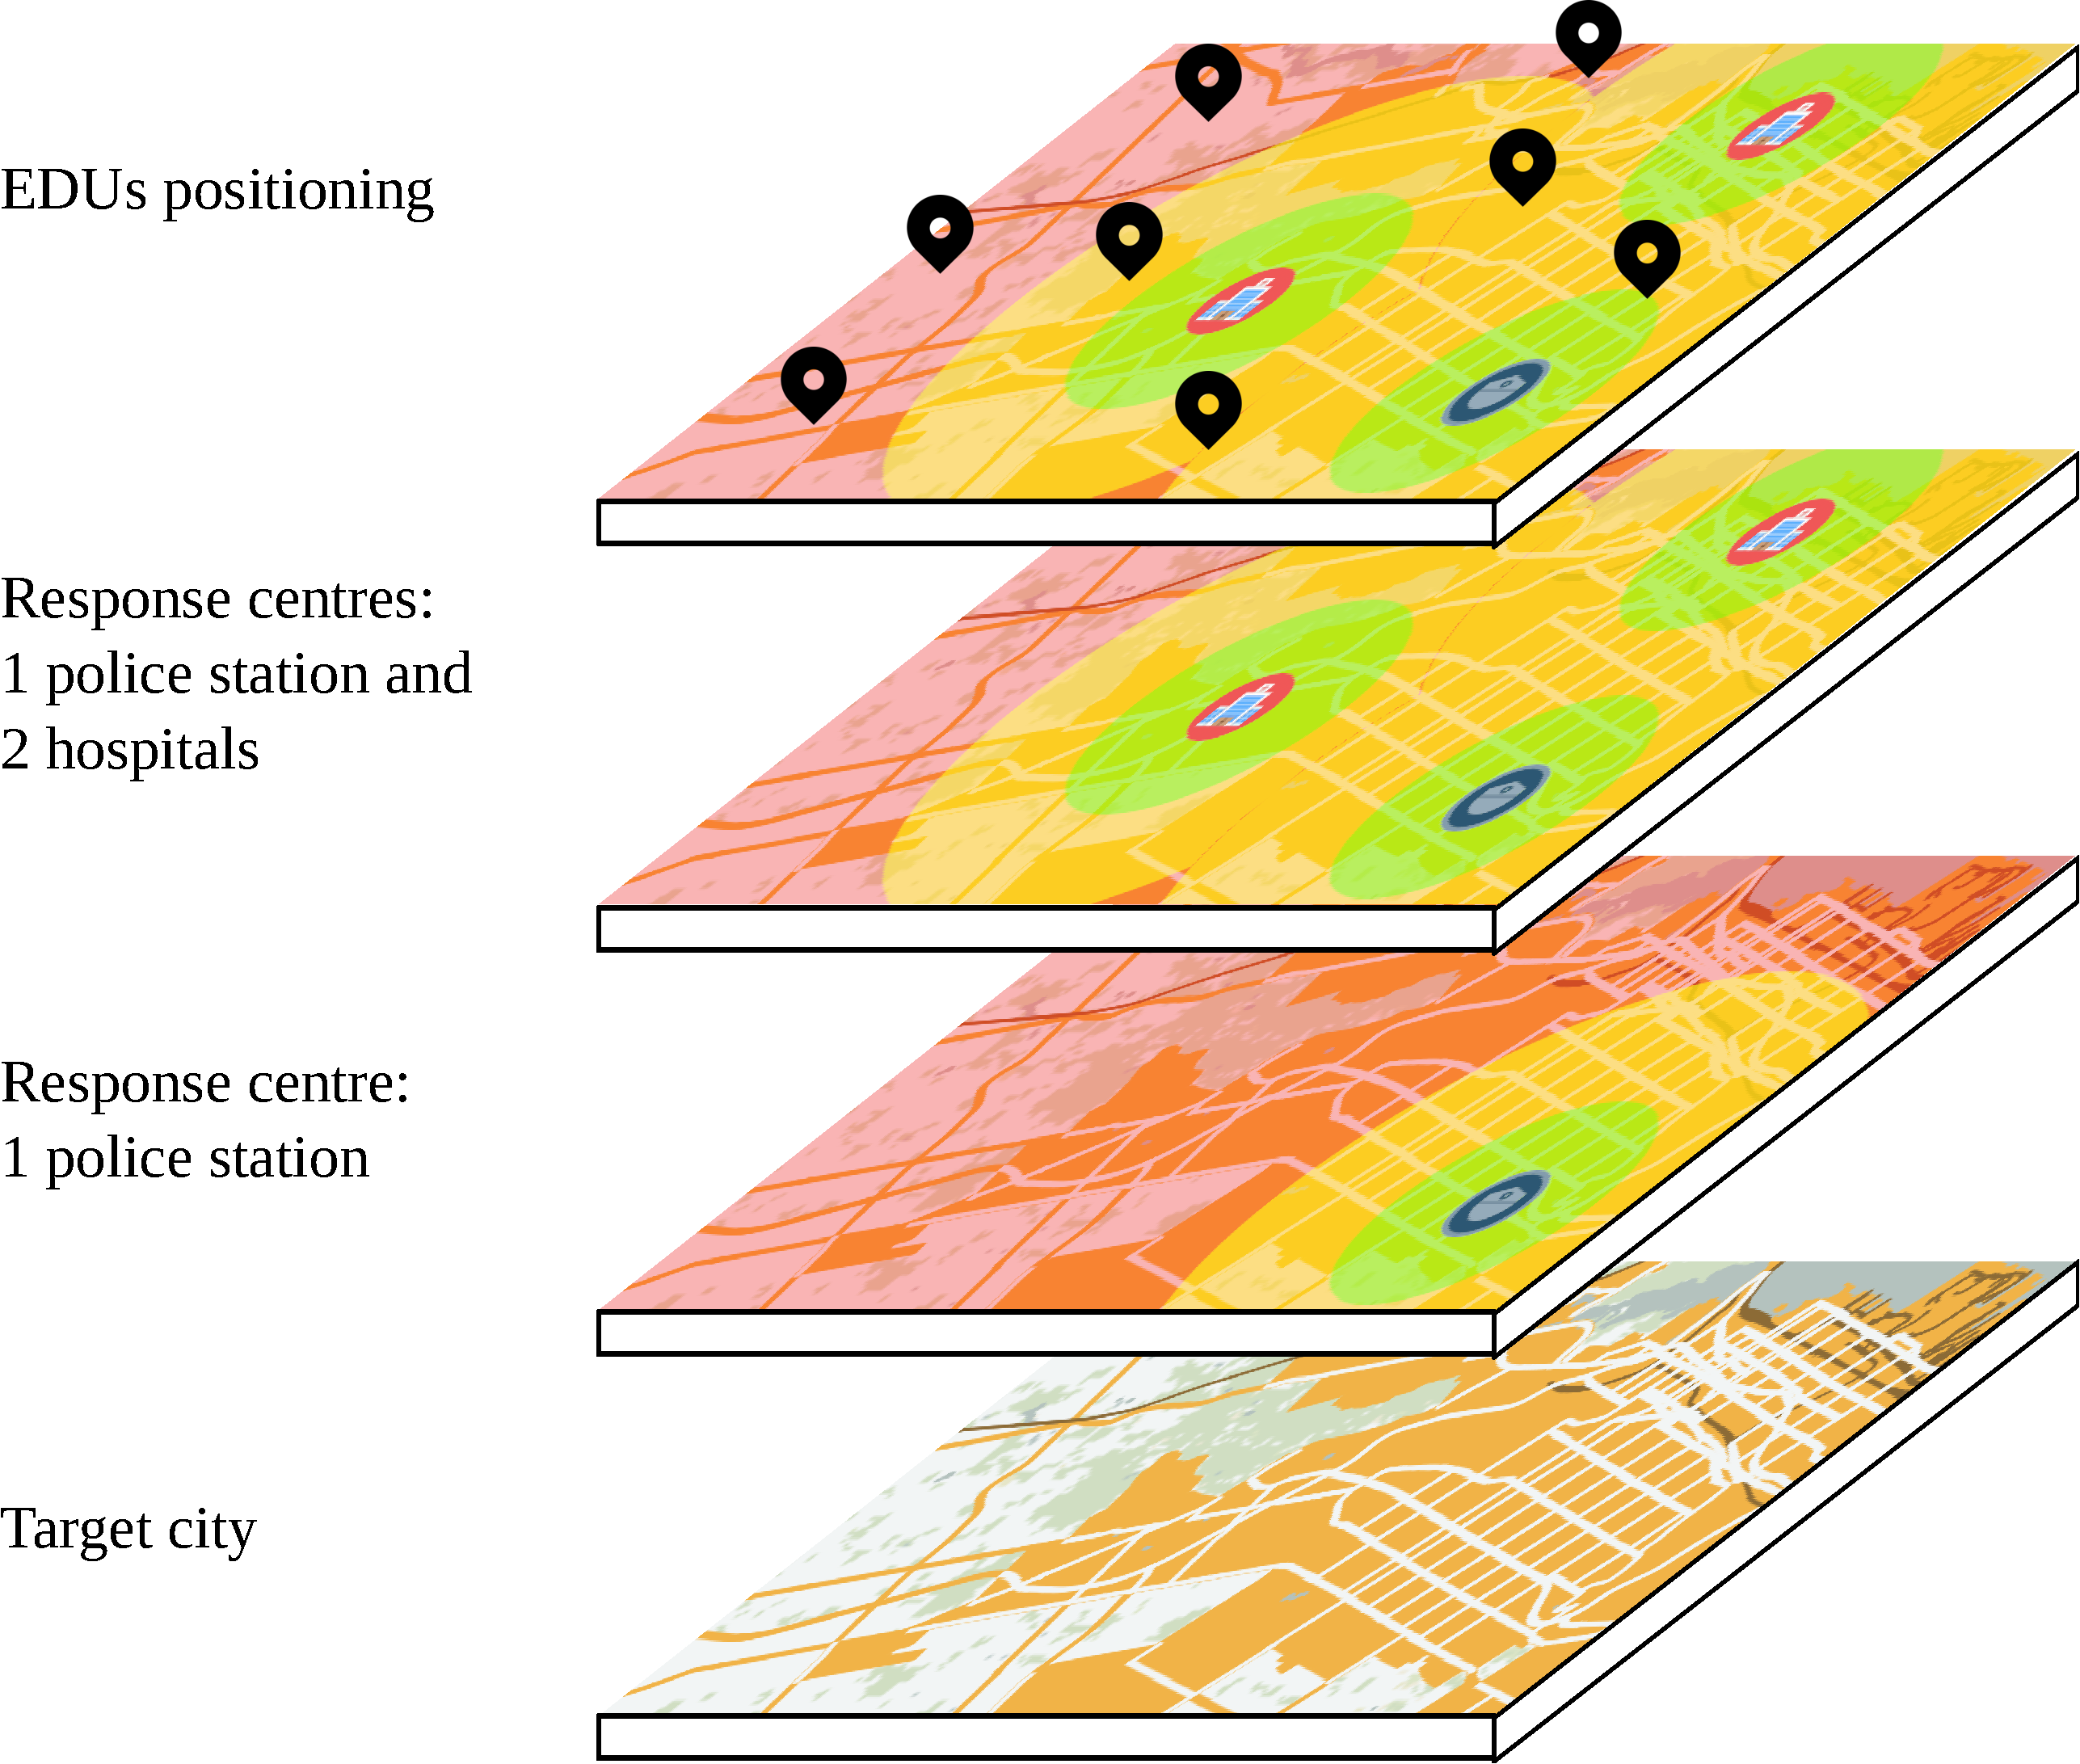
\includegraphics[width=0.7\linewidth]{Chapters/2-EDUs/images/map_layers.pdf}
    \caption{A conceptual representation for the definition of mitigation zones in a city.}
    \label{fig:smartcity}
\end{figure}

Therefore, considering the complexities of the presented challenges and the relevance of emergencies detection and mitigation for the creation of more sustainable and resilient cities, the contributions of this article are threefold, being described as follows:

\begin{itemize}
    \item Mathematical definitions for the concepts of Area of Influence, Mitigation Zone and Point of Interest, as well as the formulations to compute the severity indexes;
    \item The proposal of four EDUs positioning algorithms, with different expected results and costs;
    \item Experimental evaluations of EDUs positioning in two real cities, for different algorithms and input parameters.
\end{itemize}

The remainder of this article is organized as follows. Section \ref{S:2} presents related works in this area. The proposed mathematical model to compute mitigation zones and PoIs is described in Section \ref{S:3}. Section \ref{S:4} presents the four proposed EDUs positioning algorithms. Section \ref{S:5} brings experimental results and performance assessments. Final discussions and future directions are stated in Section \ref{S:6}. At last, conclusions and references are presented.

%%%%%%%%%%%%%%%%%%%%%%%%%%%%%%%%%%%%
\section{Related works}
\label{S:2}

This work is concerned with algorithms to compute suggested deployment positions for multi-sensor Emergencies Detection Units (EDUs) in a city, taking as reference the existence of response centres when defining mitigation zones. Hence, related works addressing the use of geospatial data in smart cities, as well as the positioning of sensors within an urban scenario, were reviewed and discussed, supporting the developments in this article.

A central aspect of smart cities approaches is the retrieving, processing, and storage of large amounts of data, sometimes in a real-time basis \cite{surveycity1}. When managing urban emergencies, critical data that may be associated to an emergency have to be retrieved somehow and there are some solutions in the literature employing sensors, smartphones, social media, and open databases as data sources \cite{surveycity2,emergencies1}. Among such possibilities, sensors have been employed as affordable and highly flexible resources to retrieve scalar data as temperature, humidity, luminosity, CO\textsubscript{2} concentration, among many other variables, allowing a more distributed perception of how (and where) adverse conditions may happen in a city \cite{multiSensor,surveyEmergencies2}. Moreover, scalar sensors can also be combined with cameras and microphones to enhance the perception of the sensors' surroundings with multimedia data \cite{smartcitiescameras}. As a result, the literature has already presented many technological possibilities when implementing multi-sensor emergencies detection units, creating the foundations for more comprehensive emergencies management systems. However, EDUs positioning still remains a challenge when the particularities of each city has to be properly considered.

%% geospatial data
Smart cities are naturally benefited from the adoption of geospatial data in different scales \cite{sharingservices}. The use of longitude and latitude metadata associated to information extracted from an urban context may have many advantages, supporting more realistic perceptions about the different dynamics in a city \cite{surveygps}. For that, sensors-based units have been typically embedded with Global Positioning System (GPS) devices, while crowdsensing approaches and databases storing urban-related data have been usually tagged with GPS coordinates, allowing geolocation procedures for different purposes. Since many different solutions may apply, an important issue has been to properly select geospatial data sources for the defined problem scope.

Geospatial data may be central when pursuing the expected goals for a smart city application. In \cite{Fernandez_2015}, an approach was proposed to assess the urban vulnerability to flooding on parishes, specially considering old buildings in the city of Vila Nova de Gaia, Portugal. For that, information about population and buildings were considered when computing vulnerability levels, taking for that the positions of the parishes. For the work in \cite{Hondula_2015}, authors collected historical information of heat-related mortality, which are associated to data of existing urban infrastructure. In both works, socio-economic factors were associated to geospatial data, which has been a common approach in smart city initiatives.

Some works have been concerned with the processing of historical or real-time geospatial data from external databases \cite{realtimegis}, since such data could be exploited when making inferences. In \cite{uberdata1}, data from the Uber mobility service were exploited as an indirect indicator of the urban ``liveability'' of a city. In that work, the Estimated Time of Arrival (ETA) provided by an Uber API was correlated with some quality of life indicators, and thus such data could be used to create liveability maps for the target city. In \cite{openstreetmap2}, the OpenStreetMap open database was used to enhance the definition of local climate zones in cities, once more realistic urban data can be considered. In a different way, the work in \cite{googlemaps} exploited the Google Maps crowdsourcing tool to support the assessment of traffic conditions in a city.

In general, although previous works have highlighted the opportunities for geospatial data processing in smart cities when exploiting external databases, such works may be restricted by copyright issues and restrictions on data availability. This way, there is a trend to adopt open databases provided by governments and the inhabitants \cite{opendatabase1}, with living labs \cite{livinglab} and collaborative approaches \cite{cityspeed} having an important role in this trend. In this scenario, the OpenStreetMap open collaborative database has stood up, being considered as the main data source for many smart city approaches. 

%% positioning
The major objective of this article is to position emergencies detection units in a smart city, potentially assuring higher detection efficiency for a finite set of available units. To achieve that, geospatial data will be used to guide the positioning of EDUs, with open databases having an important role for this. Actually, some previous works have proposed different approaches to support the positioning of sensors in a city, influencing this work in different ways. In \cite{positioning1}, authors considered the roads map obtained from OpenStreetMap, as well as wireless connectivity issues, when positioning a set of sensors nodes, which resulted in the definition of deployment graphs. In that work, the transmission range was considered as an important input parameter for the placement of the nodes. In \cite{positions2}, some fixed multi-sensor units were used to complement data retrieved by a crowdsensing approach, with the actual positions of those fixed units being determined by experts in the target city of Porto, Portugal. Particularly, the defined positions of the units in that work took as reference the traffic, parking, residential, and touristic characteristics of the areas in the considered city. In a different way, authors in \cite{positioning3} considered the transmission range and the position of multiple sinks when positioning sensor nodes, without particular regard to the actual infrastructure and geographical characteristics of a city. These works are examples of how different geospatial data can be leveraged when positioning sensor nodes.  

At this point, it is important to note that geospatial data can be retrieved from different sources, with particular challenges to be handled. In some cases, data can be retrieved from social media \cite{twitterGeospatialSensors}, once latitude and longitude coordinates can be associated to public online posts. Additionally, crowdsensing applications can be used to support sensors deployment when positions of the contributing sources can be properly known \cite{positioning5}. In this article, OpenStreetMap is exploited to provide data about the roads and streets, as well as data of response centres within the considered urban area. Although different types of response centres could be considered, since the proposed mathematical model is flexible to encompass any type of Point of Interest, the performed experiments were concerned with hospitals, fire departments, police stations/posts, and mobility hubs (metro stations), which are very common in modern cities. 

%% Table
Table \ref{Table:related} summarises previous works in the literature, highlighting the employed source of geospatial data. 

\begin{table}
    \centering
    \caption{Some works exploiting geospatial data to support sensors positioning and deployment.}
    \label{Table:related}
    \begin{tabular}{|c|c|c|c|}
        \hline
        \textbf{Work} & \textbf{Data source} & \textbf{City} & \textbf{Objective} \\ 
        \hline
        \cite{positioning1} \cite{positioning1}  &  OpenStreetMap & many, Turkey & Roads monitoring\\ 
        \hline
        \cite{positions2} \cite{positions2}  & Experts in the target city & Porto, Portugal & City livinglab \\ 
        \hline
        \cite{positioning3} \cite{positioning3} & Simplified geographical area & New York, USA & Generic sensing \\ 
        \hline
        \cite{twitterGeospatialSensors} \cite{twitterGeospatialSensors} & Social media & New York, USA & Sensors calibration \\ 
        \hline
        \cite{positioning4} \cite{positioning4} & Group of existing buildings & Santiago, Chile & Monitoring of particulate matter \\ 
        \hline
        \cite{positioning5} \cite{positioning5} &  OpenStreetMap & Seoul, South Korea & Air quality monitoring \\ 
        \hline
    \end{tabular}
\end{table}

%%%%%%%%%%%%%%%%%%%%%%%%%%%%%%%%%%%%%%%
\section {Fundamental concepts and mathematical model}
\label{S:3}

The positioning of emergencies detection units in a target city will be guided by the presence of response centres, taking as reference their geospatial metadata and existing urban infrastructure. The response centres will be considered when defining mitigation zones, which is a proposed concept to mathematically support the positioning of any number of EDUs in any urban area. 

This article defines processing steps to be followed, both for the required mathematical modelling and for the positioning algorithms, as depicted in Figure \ref{Fig:figFluxograma}. The processing steps are presented along with the associated data sources and formats, highlighting the complete processing cycle of the proposed approach. The steps 1, 2 and 3 are described in this section.

\begin{figure}[htb!]
    \centering
    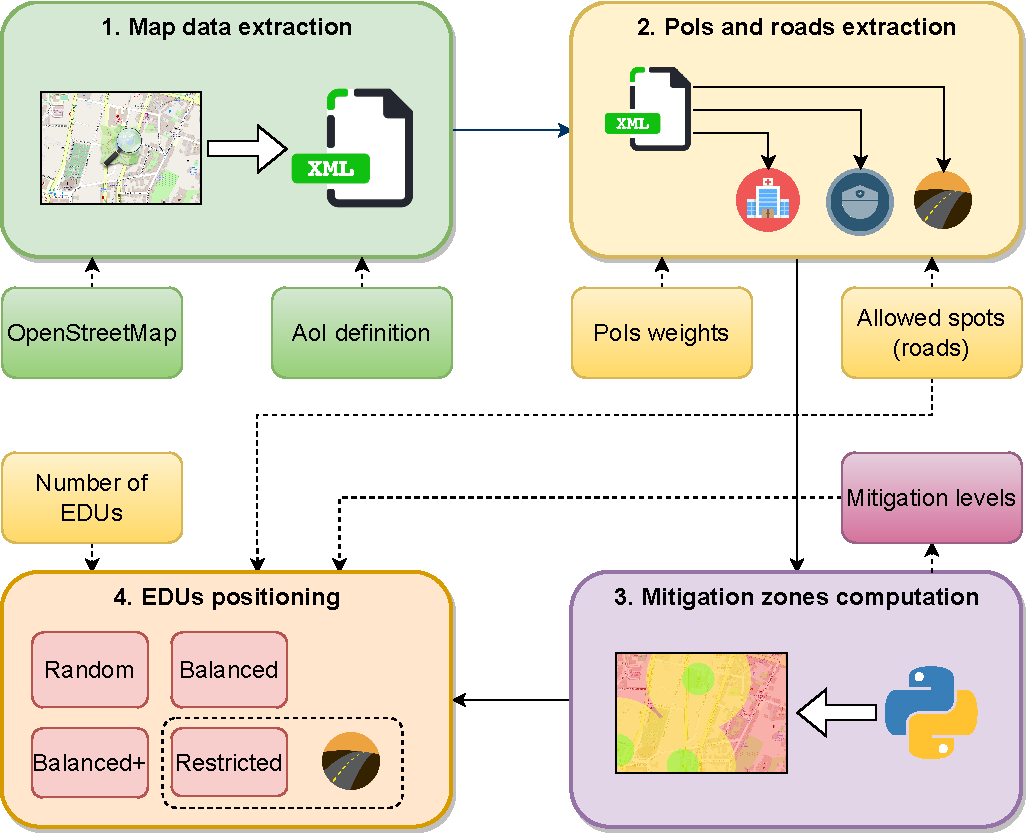
\includegraphics[width=0.85 \linewidth]{Chapters/2-EDUs/images/flowchart.drawio.pdf}
    \caption{The processing flow and data interactions in the proposed EDUs positioning approach.}
    \label{Fig:figFluxograma}
\end{figure}


%%
\subsection{OpenStreetMap and Points of Interest}

The availability of digital map databases to provide geospatial data about geographical elements on the ground has supported the development of different applications, with special attention to smart city projects \cite{spatial2,spatial1}. Among the available databases, OpenStreetMap (OSM) stands out as a crowdsourced geographic information database that is supported by collaborative work from volunteers worldwide \cite{openstreetmap}. This way, the maps are freely available for visualisation, query, download, and modification, being a powerful data source with no copyright restrictions. Additionally, as the users community can adapt the maps to quickly comply with changes in the real world, it is expected that the available information will be often reliable and up-to-date. Finally, a considerable number of flexible APIs are available for many programming languages, facilitating the retrieving and processing of geospatial data from this database.

In short, OSM defines a conceptual data model of the physical world, representing features on the ground like roads and buildings through the definition of ``nodes'', ``ways'', and ``relations''. Doing so, metadata are associated to the modelled elements, providing valuable data for different types of applications.

Among the available data in the OpenStreetMap database, response centres can be identified when searching queries are properly executed. As mentioned before in this article, the resilience of an area within a city will be associated to the presence (and distances) to response centres. Then, in a different way from previous works, we propose to compute the severity level of the mitigation zones (described latter in this section) based on the presence of such response centres, each one defined as a Point of Interest (PoI).

Actually, a city may have different types of response centres, which are some kind of urban infrastructure that may be associated to mitigation actions that would be triggered after the detection of an emergency \cite{surveyEmergencies}. In this context, for example, if an emergency happens near a hospital, there is a better chance to attend victims on time, and the same is true for a fire incident not far from firefighters. The challenge is then to identify such ``points'' and to extract their GPS coordinates, which can be retrieved from OpenStreetMap (or other geospatial database) using proper keywords. 

Hence, there will be $P$ points of interest, regardless of their types (e.g. hospitals, fire departments, bomb shelters, metro stations, helipads, police posts, etc), since we do not differentiate their roles when responding to a detected emergency, although we define four basics types of response centres for benchmark. Actually, a PoI is identified when it has some important role for emergency mitigation, either supporting direct response actions like dispatching ambulances or firetrucks, or supporting indirect actions like rescuing procedures and evacuation from affected areas.

Whatever is the defined list of points of interest, a PoI $p_j \in P$ will be associated to a weight function $f(p_j)$ to indicate how relevant is that infrastructure in a city (e.g. large hospitals may be more relevant than small ones), which is a subjective aspect of the proposed approach that allows some level of ``calibration'' to the particularities of a target city.

%
\subsection {Defining mitigation zones}

A Mitigation Zone (MZ) is the core element when guiding the positioning of EDUs. Overall, a city may have different numbers and configurations of MZ, depending on the considered parameters. For that, the first step when modelling mitigation zones is the definition of an Area of Influence (AoI), which is a geographical area that may sprawl beyond a city and comprise areas from different parts of a metropolitan area. Actually, since it is very common to have ``clusters'' of cities that create a continuous urban area, it is reasonable to consider a target AoI instead of a single city. 

An AoI will be modelled as a rectangle delimited by a top-left vertex at the ($A_x$,$A_y$) coordinates (latitude and longitude) and a bottom-right vertex at the ($B_x$,$B_y$) coordinates, which can be freely defined according to any constraint. This modelled rectangle can be perceived as a 2D plane, but Haversine distances will always be taken when needed (instead of Euclidean distances). 

The defined AoI will be divided into contiguous and disjointed square-shaped subareas referred as mitigation zones, each one with a known physical position and having the same dimensions (width/height of the defining square). Since there will be a set $Z$ of mitigation zones for an AoI, with each zone $z_i \in Z$, it is possible to define that a mitigation zone $z_i$ will be positioned at ($x(z_i)$,$y(z_i)$) coordinates, having a with of $l$ meters, and a mitigation level of $ML(z_i)$, for $0 < i \le |Z|$. The adoption of mitigation zones as squares can reduce the computational cost while still assuring reasonable accuracy, specially when small zones are defined. The total area of the resulting grid-like AoI can be computed by summing up the areas of all mitigation zones' squares.

The adopted approach of using configurable squares when defining the zones results in the fact that the value of $|Z|$ (the total number of mitigation zones) will directly depend on the chosen value for $l$. While larger zones are faster to compute, it is expected that the achieved accuracy will increase for shorter zones, giving flexibility when adopting the proposed approach. This way, the highest accuracy would be achieved when defining mitigation zones as single GPS coordinates, but the achieved outcome may not justify the additional computational cost in some cases. 

The value of $|Z|$ can be computed as presented in Equation \ref{eqZones}. The function $dist(pointA, pointB)$ computes the distance between the provided points using the Haversine formula, which returns more accurate distances when GPS coordinates are adopted. 

\begin{equation}
    \begin{split}
        \displaystyle Z_w &= \left\lfloor \frac{dist(A_x,B_x)}{l} \right\rfloor\\
        \displaystyle Z_h &= \left\lfloor \frac{dist(A_y,B_y)}{l} \right\rfloor\\
        \displaystyle \lvert Z \rvert &= Z_w \cdot Z_h\\
    \end{split}	
    \label{eqZones}
\end{equation}

Equation \ref{eqZonesPoints} defines the computing of the coordinates of any mitigation zone $z_i$, assuming \textit{mod} as the modulus of an integer division, and $i$ as an index within the $Z$ set.

\begin{equation}
    \begin{split}
        \displaystyle x(z_i) &= A_x + l \cdot (i\ mod\ Z_w)\\
        \displaystyle y(z_i) &= A_y + l \cdot \left(\left\lfloor \frac{i}{Z_w} \right\rfloor\right)\\
    \end{split}	
    \label{eqZonesPoints}
\end{equation}

Then, the centre point of the zones can be computed, defined as the $(x_c(z_i),y_c(z_i))$ coordinates, as presented in Equation \ref{eq1}. These coordinates are required when computing the mitigation levels of the zones.

\begin{equation}
    \begin{split}
        \displaystyle x_c(z_i) &= x(z_i) + \frac{l}{2}\\
        \displaystyle y_c(z_i) &= y(z_i) + \frac{l}{2}\\
    \end{split}	
    \label{eq1}
\end{equation}

At this point, the mitigation zones of an AoI are correctly modelled and ready to be processed. However, it is reasonable to incorporate the particularities of the modelled urban area, even though an AoI is mathematically defined as a rectangle. For example, the AoI rectangle may cover parts of a river or the sea that may not be regarded as areas for the deployment of EDUs. This way, mitigation zones may be removed from the set $Z$ during an additional processing step, using the limits of a city (or other parameter) as reference, although the set of considered rescue centres is not changed in this case. Actually, the OpenStreetMap allows the indication of the contours of any city, facilitating this process. Whatever the case, we expect that this additional processing step would not compromise the expected results of the proposed approach as a whole.

Figure ~\ref{Fig:figGrid} graphically presents the definition of mitigation zones.

\begin{figure}[htb!]
    \centering
    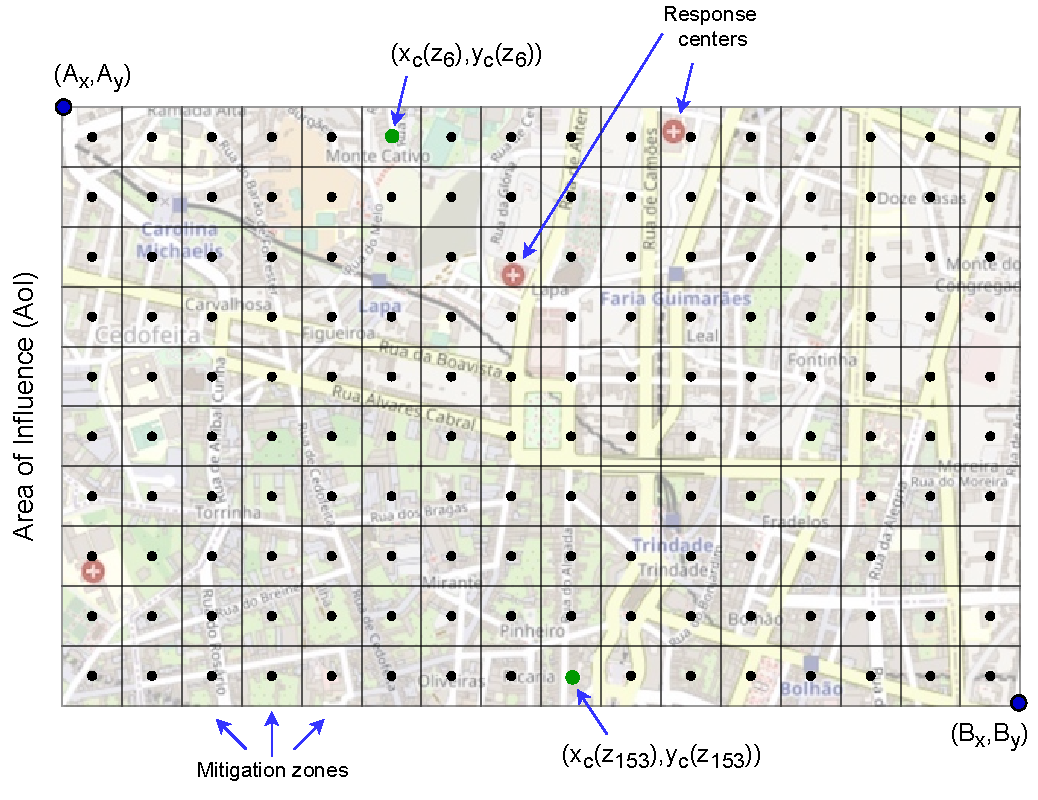
\includegraphics[width=0.77\linewidth]{Chapters/2-EDUs/images/MitigationZones.pdf}
    \caption{An example with 160 mitigation zones defined for an area of influence.}
    \label{Fig:figGrid}
\end{figure}

%
\subsection {Computing the mitigation levels}

Each mitigation zone will be tagged with a mitigation level, a numerical index within a previously defined range. The computation of the mitigation level of a zone ($ML(z_i)$) will happen after the definition of the list of PoIs and mitigation zones, being the last step before the positioning of the EDUs. 

The mitigation level of the zones will be computed based on an indirect relation between geographical areas and urban hazards and emergencies. Actually, to strongly associate hazards to the mitigation levels of zones may be too hard to achieve, demanding specific knowledge of a city or even taking other complementary data that may be not openly available. In a different way, we propose to consider the resilience to untreated emergencies according to the available urban infrastructure, which is easier to be mathematically processed in a more generic way \cite{emergencies1}. As discussed before, such resilience is indirectly accounted by taking the list of Points of Interest within the AoI.

Therefore, the higher the likeability of a region (and people) to recover from an emergency supported by existing PoIs, the higher is its resilience. This way, the balanced proximity of a zone $z_i$ to mitigation-related facilities (response centres) will indicate its mitigation level. As discussed before, different types of points of interest may be defined for an urban area, as long as their GPS coordinates are known.

Initially, it is performed the summing up of the squared distances from each zone to every PoI $p_j \in P$, multiplied by its weight factor $f(p_j)$. We adopt a weight factor to define the importance level of each PoI within an urban area, since some PoI may have higher importance during mitigation actions (e.g. larger hospitals or fire departments with better equipped trucks). Equation \ref{eq:risk_level} defines the performed computation in this processing step, for $E(z)$ as the combined risk perception of zone $z$ and $dist:Z,P~\to~\mathbb{R^+}$ as the distance function from a zone to a PoI.

\begin{equation}
    \label{eq:risk_level}
    E(z_i) = \cfrac{1}{\displaystyle\sum_{j = 1}^{\lvert P \rvert}\left(\cfrac{1}{dist^2(z_i, p_j)} \cdot f(p_j)\right)} 
\end{equation}

After computing the risk perceptions, the mitigation levels of each zone can be computed. This way, it is defined that $ML(z_i) \in M$, with $M$ as a set of ordered consecutive positive integers starting from $1$ until $|M|$: since the set $M$ is configurable, the value of $|M|$ will indicate how many different mitigation levels are being considered. Equation \ref{eq:risk_class} presents the computation of $ML(z_i)$, with $ML(z_i)~=~1$ as the lowest mitigation level and $ML(z_i)~=~|M|$ as the highest level. Additionally, $ML:Z \to \mathbb{N}$ is defined as the mitigation level classification function of a zone $z_i$, for $\widehat{E}$ as the normalisation of the risk perception function $E(z_i)$. 

\begin{equation}
    \label{eq:risk_class}
    ML(z_i) = M - \min\left(M - 1, \left| \left\lceil \ln{\widehat{E}(z_i)} \right\rceil \right| \right)
\end{equation}

As an important remark, the classification of each zone as being in one of the possible mitigation levels is relative to the region being considered. In other words, a zone is as risky as other zone with the same mitigation level if they belong to the same defined AoI, and thus it is meaningless to perform comparisons of zones if they are processed within different areas of influence. 

An additional consideration in Equation \ref{eq:risk_class} is that a natural logarithmic computation is performed when achieving the risk levels of the zones. In fact, different bases for the logarithm function could be adopted, with different final results for the zones, but it has been common in the literature to adopt natural logarithms (base $\mathrm{e}$) when computing classes and groups for different urban variables, particularly due to its mathematical properties \cite{log3,log4,log1,log2}.

Figure \ref{Fig:figGrid2} depicts a visual example of an AoI after computation of the mitigation levels. 

%\vspace{-3cm}
%\setlength{\textfloatsep}{0pt}

\begin{figure}[htbp!]
    \centering
    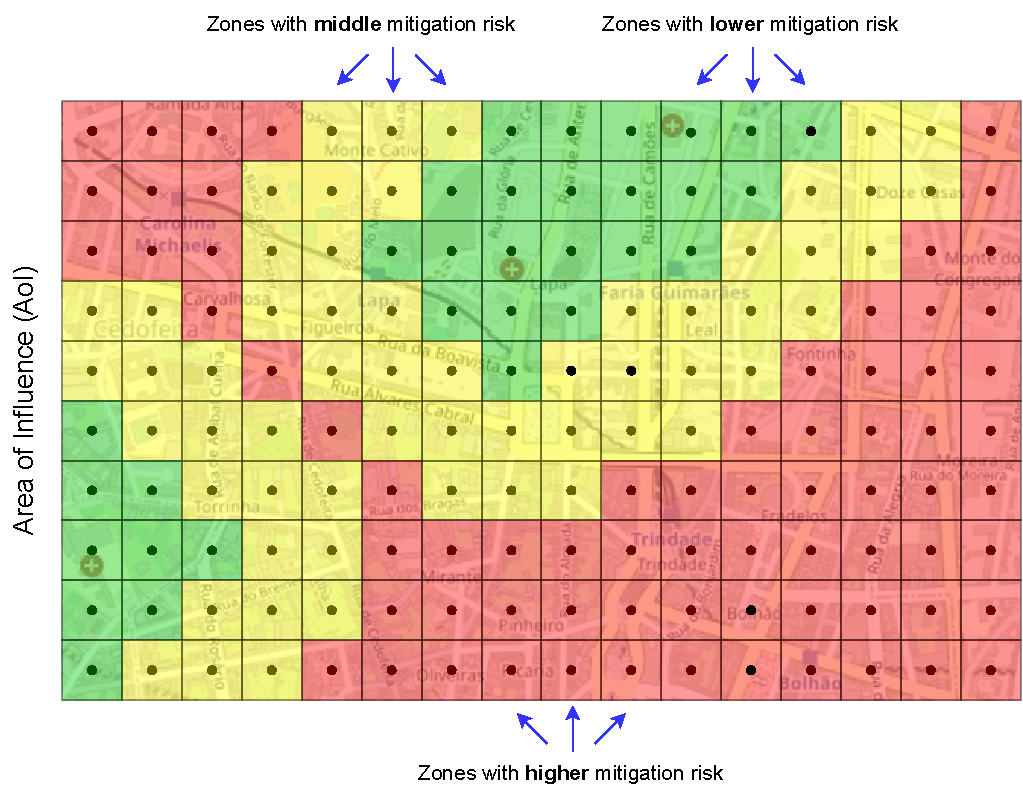
\includegraphics[width=0.77\linewidth]{Chapters/2-EDUs/images/MitigationZonesColors.pdf}
    \caption{An example of zones after computing the mitigation levels, for $|M|=3$ and 3 considered points of interest.}
    \label{Fig:figGrid2}
\end{figure}

In the example in Figure \ref{Fig:figGrid2}, $|M|=3$ and a grid of $16~\times~10$ mitigation zones is defined. Since we adopt a similar pattern of common heatmaps, it is defined that $ML(z_i)~=~1$ is green, $ML(z_i)~=~2$ is yellow, and $ML(z_i)~=~3$ is red, when plotting on a map for $|M|=3$.


%%%%%%%%%%%%%%%%%%%%%%%%%%%%%%%
\section{Proposed positioning algorithms}
\label{S:4}

After the computation of the mitigation level ($ML$) of each zone within the defined AoI, the geospatial risk perception can be now mathematically computed. With this information, the step 4 of the flowchart depicted in Figure \ref{Fig:figFluxograma} can be executed. Actually, in this next step of the proposed approach, different algorithms might be applied, with different complexities and expected results. 

A total of four different EDUs positioning algorithms are proposed in this work. In general, the proposed algorithms have to compute how many EDUs will be allocated to each mitigation level in order to better monitor the zones and reduce the average impacts of emergencies. For that, since zones with higher $ML$ will be potentially harder to be assisted by emergency response actions due to their proportional distance to the existing PoIs, those zones should be better covered by EDUs in order to prioritise critical events detection in such less assisted areas. In other words, it is intended to prioritise zones with higher computed risk in order to achieve a better behaviour on average, proportionally better covering areas that would be worst affected by emergencies. Doing so, we expect to potentially achieve a fairer emergency-centred smart city service by not neglecting areas in a city that are already badly assisted by public services. The challenge is then how to distribute the selected EDUs for the mitigation levels, with different options available for that.

Whatever is the chosen strategy, the proposed algorithms do not compute the ideal number of EDUs required to cover the entire AoI. Instead, governmental entities and urban stakeholders must indicate the number of available EDUs for deployment, leaving the positioning decisions to the algorithms. This way, for the total number of EDUs defined as $U$, the number of EDUs in each zone is computed as defined in Equation \ref{eq:classes_distribution}.

\begin{equation}
    \label{eq:classes_distribution}
    \begin{split}
        \displaystyle n_m &= \frac{U}{\displaystyle\sum_{h = 1}^{|M|}\left(h \cdot a_h\right)} \cdot (m \cdot a_m)
    \end{split}
\end{equation}

Equation \ref{eq:classes_distribution} calculates the number $n_m$ of EDUs in each level $m$ in order to create a proportional distribution of sensing units, considering the total area $a_m$ of each level, prioritising zones with higher mitigation levels while restricting the total number of EDUs to $U$ units. After the computation of the number of EDUs in each mitigation level, an algorithm sets the position of every unit within the AoI. Depending on the chosen algorithm, the number of selected EDUs may vary around the value of $U$. That happens because the provided value for $U$ may not be suitable to fulfil the whole AoI according to a criteria defined by each algorithm.

Four proposed positioning algorithms are described in this section: \emph{Random}, \emph{Balanced}, \emph{Balanced+} and \emph{Restricted}. Each algorithm follows a particular positioning approach, presenting different computational costs. In a general sense, every proposed algorithm is an improvement of the former one, making the Restricted algorithm the more realistic and potentially most adequate for real-world scenarios.

\subsection{Optimising the coverage area}

For better detection of emergency events, the EDUs must cover the larger area possible inside the AoI. If there are enough units to be deployed in a way that every zone can be reached by at least one of them, we have a full coverage distribution, but this is not always the case. Our approach takes into consideration the fact that the EDUs are a limited resource and depending on the AoI size it will not be possible to have units enough to cover the whole area. This raises an optimisation problem, which is: given some restrictions, we must maximise the coverage area of the sensing units through a positioning schema. These considerations are stated as follows.

\begin{itemize}
    \item Restrictions:
    \begin{enumerate}
        \item Total number of EDUs ($U$);
        \item Number of EDUs per mitigation level ($n_m$).
    \end{enumerate}
    \item Goal: to maximise the overall coverage area of the AoI by the EDUs.
\end{itemize}

In this process, the EDUs must be distributed in an equidistant manner, spreading over the whole AoI as possible. The restrictions limit the number of EDUs in the whole AoI as also per mitigation level in order to obey the proportion distribution presented in this section. Thus, placing the EDUs in an equidistant manner will provide the best coverage solution as long as every EDU has the same sensing radius. Placing the EDUs too close to each other will create overlapping zones, reducing the coverage area. Such overlapping may happen in some situations depending on the area of the highest ML and the number of EDUs, but the equidistant positioning will always produce the scenario with less overlapping. In fact, the overlapping area of two sensing units can be obtained by calculating the area of two intersecting circumferences as shown in Equation~\ref{eq:overlapping_area}.

\begin{equation}
    I = r^2(\theta - \sin(\theta))
    \label{eq:overlapping_area}
\end{equation}

In order to maximise the coverage area, overlapping has to be minimised, and thus we have to minimise the value of $I$. Since $r$ is fixed, to minimise $I$ we must minimise $(\theta - \sin(\theta))$. The angle $\theta$ is the angle formed by the radius of any of the overlapping circumferences and the two intersection points as show in Figure~\ref{fig:circle_intersection}. This angle increases when the two circumferences get closer and decreases otherwise, thus, keeping the circumferences distant obviously reduces the overlapping area. Finally, placing the EDUs in an equidistant manner will avoid unnecessary overlapping and provide the maximum coverage possible, which guides the operation of the proposed algorithms.

\begin{figure}[htbp]
    \centering
    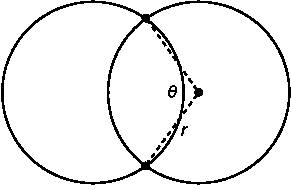
\includegraphics{Chapters/2-EDUs/images/circumferences_overlapping.pdf}
    \caption{The angle $\theta$ formed by the radius and the two intersection points.}
    \label{fig:circle_intersection}
\end{figure}

%%
\subsection {Random algorithm}

The first proposal for the EDUs follows a random positioning principle, according to the proportion ratio defined in Equation \ref{eq:classes_distribution}. The idea is that any position is valid for an EDU $z_i$ as long as the mitigation levels of the zones are considered to define deployment subsets. For example, assuming that $|M|=3$, there will 3 disjoint subsets of EDUs that may be positioned anywhere within the corresponding zone, since the combination of these 3 subsets results in the initial set of available EDUs.

The Random algorithm has the lowest computational cost, but it has no criteria for selecting the positions of the units. This way, it does not guarantee that every ``part'' of the AoI will be covered by an EDU. Actually, although it can be used to demonstrate the proportional distribution calculated in Equation \ref{eq:classes_distribution}, it is reasonable to say that this algorithm is not recommended for a real scenario of nodes deployment. 

The Random algorithm works as follows: after computing the number of EDUs per level, it randomly selects a position within the set of zones with that mitigation level for each of those EDUs. In this manner, it is possible to have several EDUs very close to each other, as well as some uncovered areas within the AoI, as defined in Algorithm \ref{alg:random}.

%%% Random algorithm
\begin{algorithm}[ht]
    \caption{Random positioning algorithm.}
    \label{alg:random}
    \begin{algorithmic}
        \REQUIRE $Z[] \gets$ the list of zones in each level, $M \gets$ number of levels, $N[] \gets$ number of EDUs needed in each level
        \ENSURE $pos[] \gets$ the list of zones that will get an EDU
        \FOR{$i$ from $1$ to $M$}
            \STATE $zones \gets random.choices(Z[i], k \gets N[i])$
            \STATE $pos[i].append(zones)$
        \ENDFOR
    \end{algorithmic}
\end{algorithm}


%%%
\subsection {Balanced algorithm}

After the definition of the mitigation zones, the Balanced algorithm calculates the EDUs coordinates within the AoI in a way that an uniform positioning distribution is achieved. This approach tries to eliminate the problems of the Random algorithm, avoiding uncovered areas and EDUs overlapping. In this sense, the Balanced algorithm calculates the coverage radius of the EDUs in each mitigation level in a way that the units are separated from each other in the same distance. The coverage radius is the distance that the units must be separated from each other in order to uniformly cover the zones with the same mitigation level. 

The Balanced algorithm computes the coverage radius in each level by dividing the total area of the zones with the same mitigation level by the number of EDUs in it, as presented in Algorithm \ref{alg:balanced}. 

%%% Balanced algorithm
\begin{algorithm}[ht!]
    \caption{Balanced positioning algorithm.}
    \label{alg:balanced}
    \begin{algorithmic}
        \REQUIRE $Z[] \gets$ the list of zones in each level, $M \gets$ number of levels, $N[] \gets$ number of EDUs needed in each level, $w, h \gets$ size of the AoI
        \ENSURE $pos[] \gets$ the list of zones that will get an EDU
        \FOR{$i$ from $1$ to $M$}
            \STATE $radius[i] \gets numpy.sqrt(Z[i] / N[i]) / 2$
            \STATE $step[i] \gets 2 * radius[i]$
        \ENDFOR
        \STATE $step_x \gets 0$
        \STATE $step_y \gets 0$
        \FOR{$y$ from $0$ to $h$}
            \STATE $step_y \gets step_y + 1$
            \FOR{$x$ from $0$ to $w$}
                \STATE $step_x \gets step_x + 1$
                \FOR{$i$ from $1$ to $M$}
                    \IF{$step_x$ mod $step = 0$ \textbf{and} $step_y$ mod $step = 0$}
                        \STATE $pos[i].append(zone(x, y))$
                        \STATE $step_x \gets 0$
                        \STATE $step_y \gets 0$
                    \ENDIF
                \ENDFOR
            \ENDFOR
        \ENDFOR
    \end{algorithmic}
\end{algorithm}

This way, it is possible to determine how the units must be set apart to cover the whole area without overlapping or creating uncovered zones. After having the coverage radius, the algorithm sequentially position every EDU in an area, creating an uniform grid of multi-sensor units.

As an important remark, although this algorithm achieves an uniform positioning, it does not guarantee coverage around the levels' borders nor avoids overlapping (between neighbour zones) in these regions.

%%%%
\subsection {Balanced+ algorithm}

The Balanced+ algorithm improves the Balanced algorithm by guaranteeing that the units are positioned correctly even in the border zones, being an enhanced version of the later. In this approach, every time an EDU is positioned, the algorithm checks if its distance from the nearest unit obeys the coverage radius that was previously calculated. In this sense, there is no overlapping in border areas and there is no uncovered areas within the AoI.

The computational cost of this algorithm is much higher than the ordinary Balanced method because of the several checks that it performs when positioning each EDU. This proposed algorithm is presented in Algorithm \ref{alg:enhanced}.

%%% Enhanced algorithm
\begin{algorithm}[ht!]
    \caption{Balanced+ positioning algorithm.}
    \label{alg:enhanced}
    \begin{algorithmic}
        \REQUIRE $Z[] \gets$ the list of zones in each level, $M \gets$ number of levels, $N[] \gets$ number of EDUs needed in each level, $w, h \gets$ size of the AoI
        \ENSURE $pos[] \gets$ the list of zones that will get an EDU
        \FOR{$i$ from $1$ to $M$}
            \STATE $radius[i] \gets numpy.sqrt(Z[i] / N[i]) / 2$
        \ENDFOR
        \STATE $smallest\_radius \gets radius[M]$
        \STATE $highest\_radius \gets radius[1]$
        \STATE $minumum\_dist \gets 2 * highest\_radius$
        \STATE $x \gets 0$
        \STATE $y \gets 0$
        \WHILE{$y < h$}
            \WHILE{$x < w$}
                \IF{$dist(zone(x, y), nearest\_edu) \leq minimum\_dist$}
                    \STATE $x \gets x + 1$
                    \STATE break
                \ENDIF
                \STATE $pos[i].append(zone(x, y))$
                \STATE $x \gets x + 2 * smallest\_radius$
            \ENDWHILE
            \STATE $x \gets 0$
            \STATE $y \gets y + 1$
        \ENDWHILE
    \end{algorithmic}
\end{algorithm}

The Balanced+ algorithm works as follows: after calculating the number of EDUs per level, it performs the coverage radius computation in the same way of the Balanced algorithm. The difference between both approaches lies on the positioning step. The enhanced Balanced+ algorithm checks if there is any other unit in the proximity of each EDU, checking if it would ``fail'' the desired coverage radius distance. If there is any other unit too close to the EDU being positioned, the algorithm moves the EDU until it gets the correct distance from its neighbours. The other change in this algorithm is related to how it positions sensing units on the borders of different mitigation levels areas. Every time the algorithm begins to calculate the coordinates for the next EDU in the Balanced algorithm, it jumps forward on the AoI the number of zones equal to the coverage radius of the units in that zone. In the Balanced+ approach, it calculates the smallest radius, i.e, the coverage radius of the highest mitigation level (where units must be closer to each other) to use as parameter to get to the next spot. Combining this approach to the computation of closer neighbour units, the enhanced Balanced+ algorithm is capable of avoiding uncovered areas in the borders of the zones.

%%%%%
\subsection {Restricted algorithm}

When considering the positioning and further physical deployment of the emergencies detection units in a city, different types of restrictions have to be properly considered in order to achieve more realistic results. For example, suppose that after the execution of the Balanced+ positioning algorithm it finds the coordinates for an EDU as being inside a private property like a residential building. In such case, although the position is indicated by the algorithm, the actual deployment may be not possible.

When the computed position for an EDU is not possible for deployment, the unit has to be positioned in another allowed place. In order to address this issue, the Restricted algorithm considers the permitted zones in an AoI to compute the positions of the EDUs, adding another restriction to our optimisation problem. 

Initially, the algorithm has to receive as input the list of allowed zones. Then, it executes the Balanced+ algorithm and uses the list of allowed zones to move the EDUs to the nearest allowed position, basically as an additional processing step. Algorithm \ref{alg:restricted} describes this operation. 

%% Restricted algorithm
\begin{algorithm}[ht]
    \caption{Restricted positioning algorithm.}
    \label{alg:restricted}
    \begin{algorithmic}
        \REQUIRE $Z[] \gets$ the list of zones in each level, $M \gets$ number of levels, $N[] \gets$ number of EDUs needed in each level, $w, h \gets$ size of the AoI, $P[] \gets$ the list of permitted zones
        \ENSURE $pos[] \gets$ the list of zones that will get an EDU
        \STATE $edus\_remaining \gets U$
        \WHILE{$edus\_remaining > 0$}
            \STATE $pos \gets balanced\_plus\_positioning(Z, M, N, w, h)$
            \FOR{$z$ in $pos$}
                \IF{$z \notin P$}
                    \STATE $pos.delete(z)$
                    \STATE $nearby\_zones \gets zones\_in\_area(z_x, z_y, 2 * z_{radius} + 1)$
                    \FOR{$nz$ in $nearby\_zones$}
                        \IF{$nz \in P$ \textbf{and} $nz$ has not an EDU}
                            \STATE $pos.append(nz)$
                            \STATE break
                        \ENDIF
                    \ENDFOR
                \ENDIF
            \ENDFOR
        \ENDWHILE
    \end{algorithmic}
\end{algorithm}

The Restricted algorithm works as follows: after running the Balanced+ algorithm, the Restricted approach visits every EDU and check if it is inside a permitted zone. If this is the case, the algorithm goes to the next EDU. If not, it finds the nearest permitted zone in the range of the coverage radius of that level to move the sensing unit to that spot. If there is a sensing unit already in the selected spot, the algorithm discards the computed movement operation. This is done because if there is an unit in that area, there is no need to have another EDU in the same spot (unless availability and redundancy are concerns to be taken). Actually, since the algorithm's input is configurable, the distance between each EDU can vary according to the number of allowed zones in the AoI. 
%In this sense, this algorithm can improve the deployment of the sensing units by saving unnecessary EDUs.

Finally, it is reasonable to expect that the Restricted algorithm has the highest computational cost because it runs the Balanced+ algorithm and then visit every unit to check if it is in an allowed zone, moving it when necessary. On the other hand, it produces the most realistic results to support physical deployment of the EDUs.

%%%%%%%%%%%%%%%%%%%%%%%%%%%%%
\section{Experiments and results}
\label{S:5}

After the definition of the mathematical model and the four EDUs positioning algorithms, different experimental scenarios were created. The performed evaluation procedures were designed to demonstrate the effectiveness of the proposed approach to position a set of EDUs, as well as to evaluate the performance of the algorithms for different input parameters. In order to achieve these results, all algorithms were implemented in the Python 3 programming language, with geospatial data being processed as XML files retrieved from the OpenStreetMap. All results are presented and discussed in this section.

%%%%%%
\subsection{Computing mitigation zones}

The computation of the mitigation zones is performed at the step 3 of the flowchart depicted in Figure \ref{Fig:figFluxograma}, when all input parameters were successfully processed in previous steps. Since a group of areas of influence was defined for this phase, different results for the mitigation zones could be evaluated. 

Initially, we considered the definition of an AoI for a big city with good urban infrastructure concerning the existence of mitigation response facilities. As defined in our proposed model, an AoI is a rectangle represented by a top-left vertex ($A_x,A_y$) and bottom-right vertex ($B_x,B_y$). The computed mitigation zones for an AoI within the city of Paris, France, at positions ($A_x = 2.279260250495456$, $A_y = 48.86514730346737)$) and ($B_x = 2.3107171978221164$, $B_y = 48.84891175843432)$), is presented in Figure \ref{Fig:zones_paris_0}, for $|M|=3$ and a list of PoIs composed of hospitals, fire departments, and police stations, all with the same relevance weight. The dimension (width/height) of each mitigation zone is defined as $l = 10m$, with this particular configuration being adopted in all experiments.

%%%%%% Zonas pra Paris, M = 3, AoI um quadrado
\begin{figure}[ht!]
    \centering
    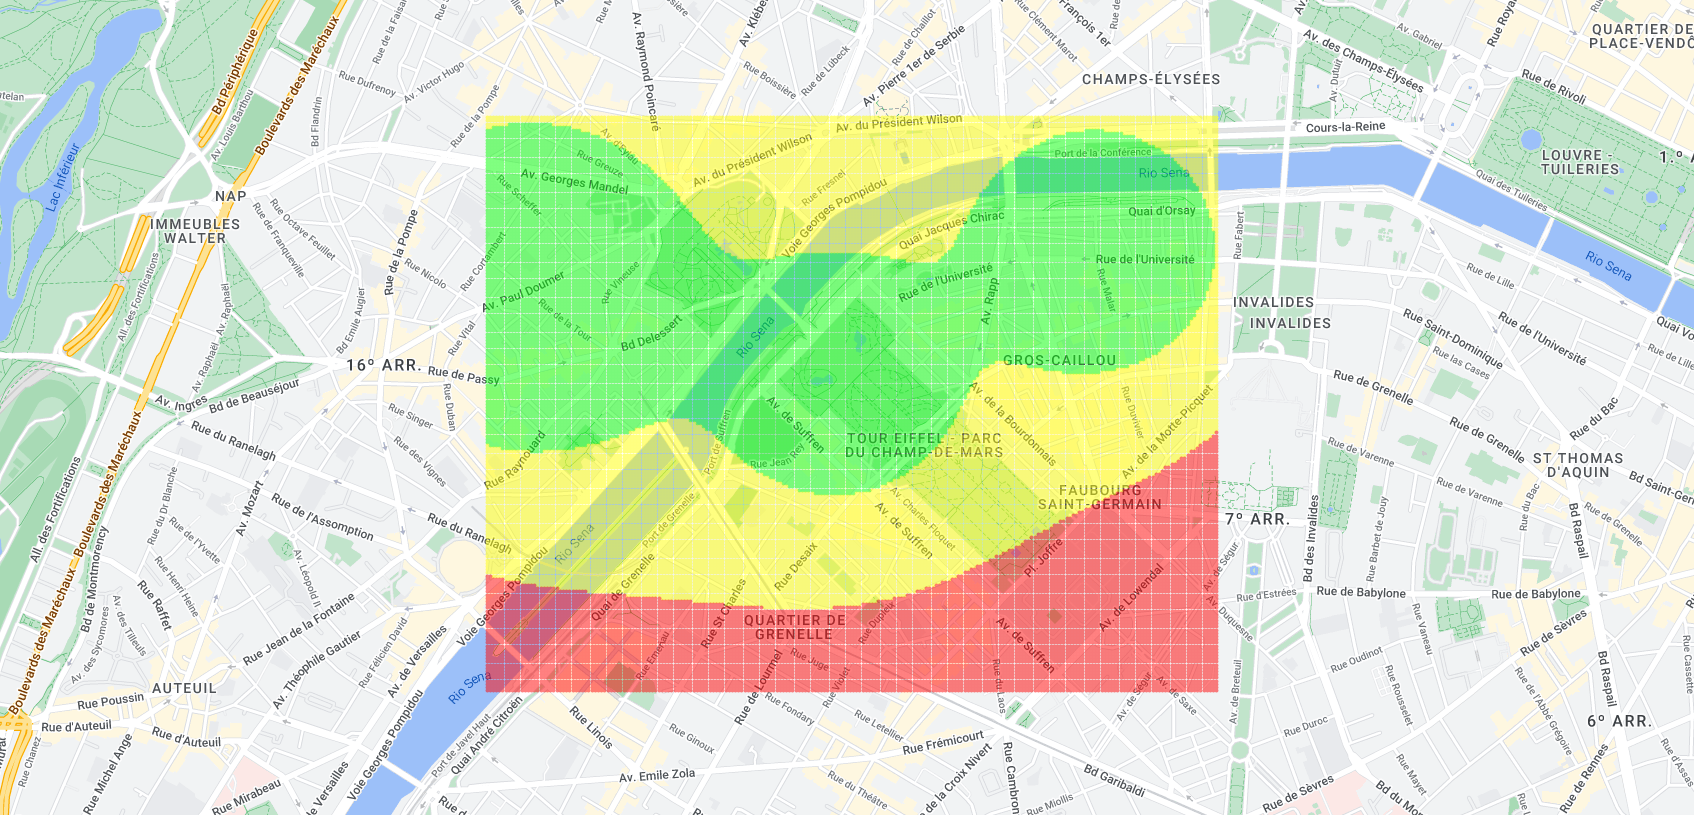
\includegraphics[width=0.9\linewidth]{Chapters/2-EDUs/images/eiffel_M3.png}
    \caption{An AoI within the city of Paris, with three different mitigation levels.}
    \label{Fig:zones_paris_0}
\end{figure}

When plotting the computed mitigation zones, it is defined that $ML(z_i)=1$ is green, $ML(z_i)=2$ is yellow, and $ML(z_i)=3$ is red. The maps are plotted using the Google Earth Engine (GEE).

As expected, mitigation zones will have a higher risk (red) when they are far from response-related urban infrastructure, considering only information extracted from the defined AoI. This fact leads us to consider bigger AoI, usually comprising at least the area of a city.

Figure \ref{Fig:zones_paris_3} presents an AoI comprising the central urban area of Paris, for $|M|=3$ and the same types of PoIs. A total of 801,241 mitigation zones was processed for $l = 10m$.

%%%%%% Zonas pra Paris, M = 3, AoI inteiro
\begin{figure}[ht!]
    \centering
    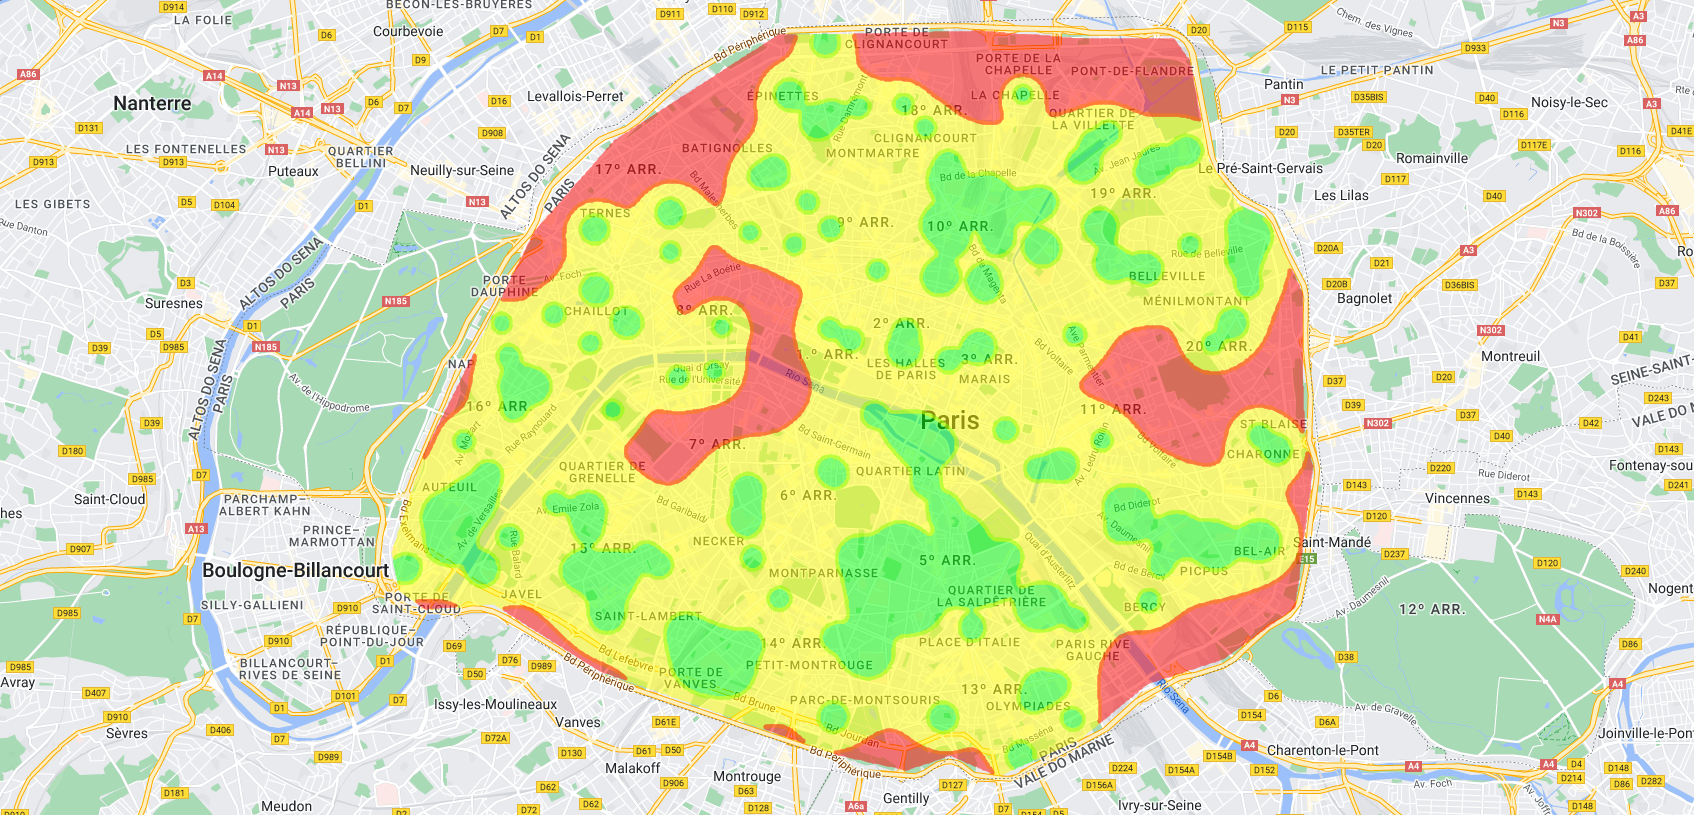
\includegraphics[width=0.9\linewidth]{Chapters/2-EDUs/images/paris_M3.png}
    \caption{A bigger AoI comprising part of Paris, with three different mitigation levels.}
    \label{Fig:zones_paris_3}
\end{figure}

It is important to remark that the definition of the AoI in this experiment started by the establishment of a rectangle that covered a large part of Paris. Then, all mitigation zones outside the defined limit (Boulevard Périphérique, a road ring) were removed, resulting in the actual AoI for processing. This particular reconfiguration was done as a pre-processing phase in step 1 of Figure \ref{Fig:figFluxograma}. In fact, this is an option that will depend on the intended modelling of a city, according to the expected level of precision (size of the zones) and processing costs. In the performed experiments, we might decide to consider the contours of the cities in order to better highlight the positioning of EDUs, but any configuration for the AoIs are possible.

%%%%%%%% Zonas pro Porto, M = 3
Still addressing the computation of mitigation zones, the city of Porto (smaller than Paris) was considered for $|M|=3$ and with a list of PoIs comprised of hospitals, police stations, fire departments, and metro stations. All PoIs are assumed to have the same weight in this experiment, in the same way of the evaluations for Paris. Figure \ref{Fig:zones_porto_3} presents the achieved result. 

\begin{figure}[ht!]
    \centering
    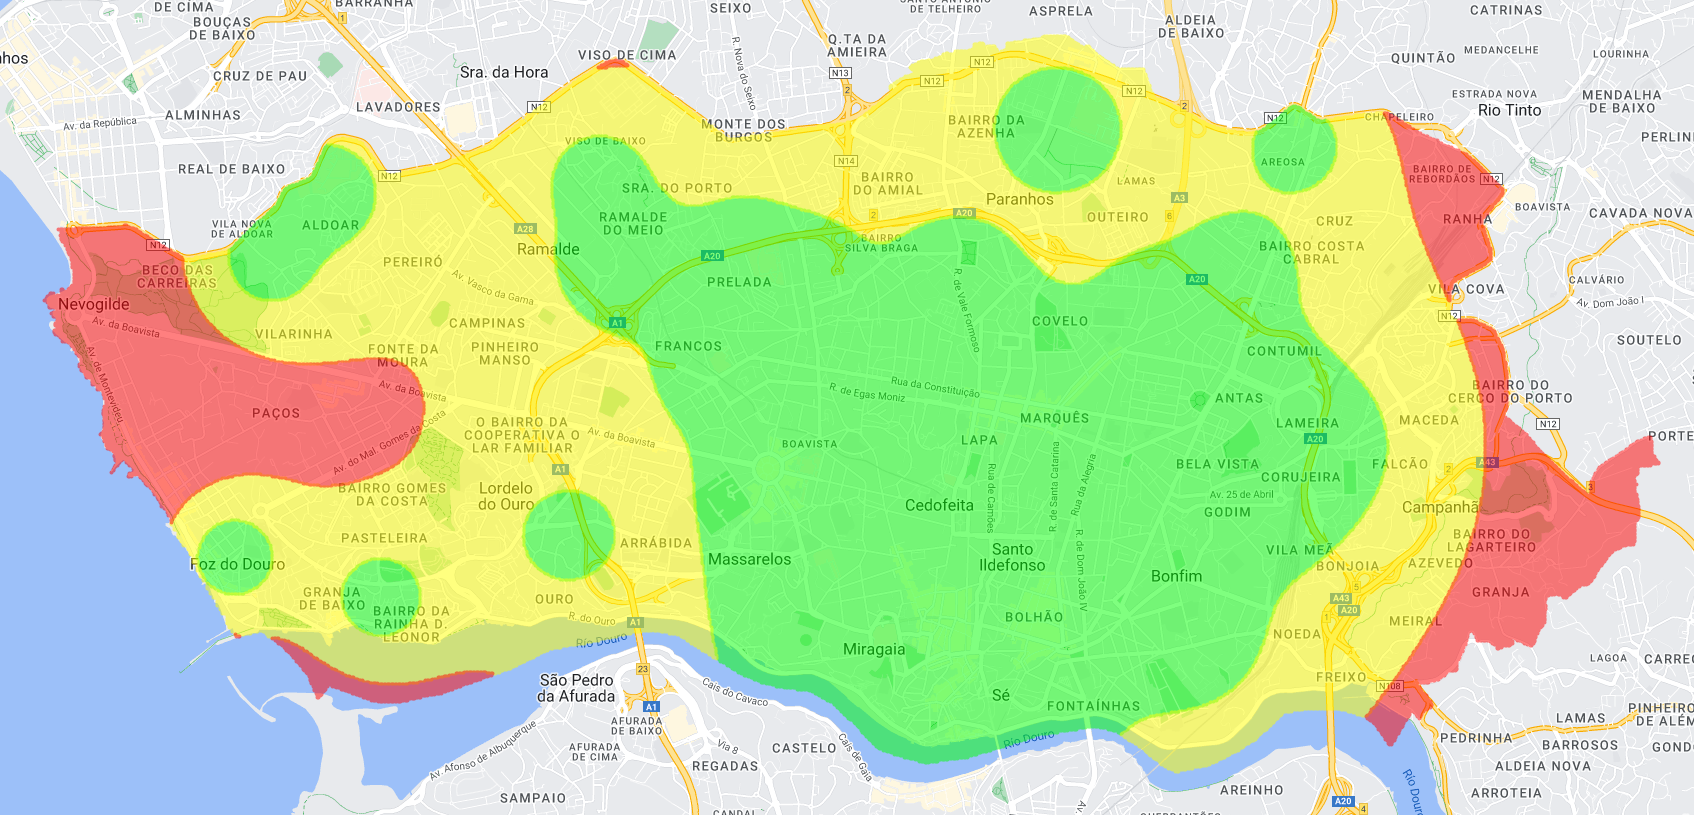
\includegraphics[width=0.9\linewidth]{Chapters/2-EDUs/images/porto_M3_no_weight.png}
    \caption{Computed zones for the city of Porto, with three different mitigation levels.}
    \label{Fig:zones_porto_3}
\end{figure}

%%%%%%% Zonas pro Porto, M = 5
Figure \ref{Fig:zones_porto_5} presents the same input parameters, but now defining $|M|=5$ for the same list of PoIs.

\begin{figure}[ht!]
    \centering
    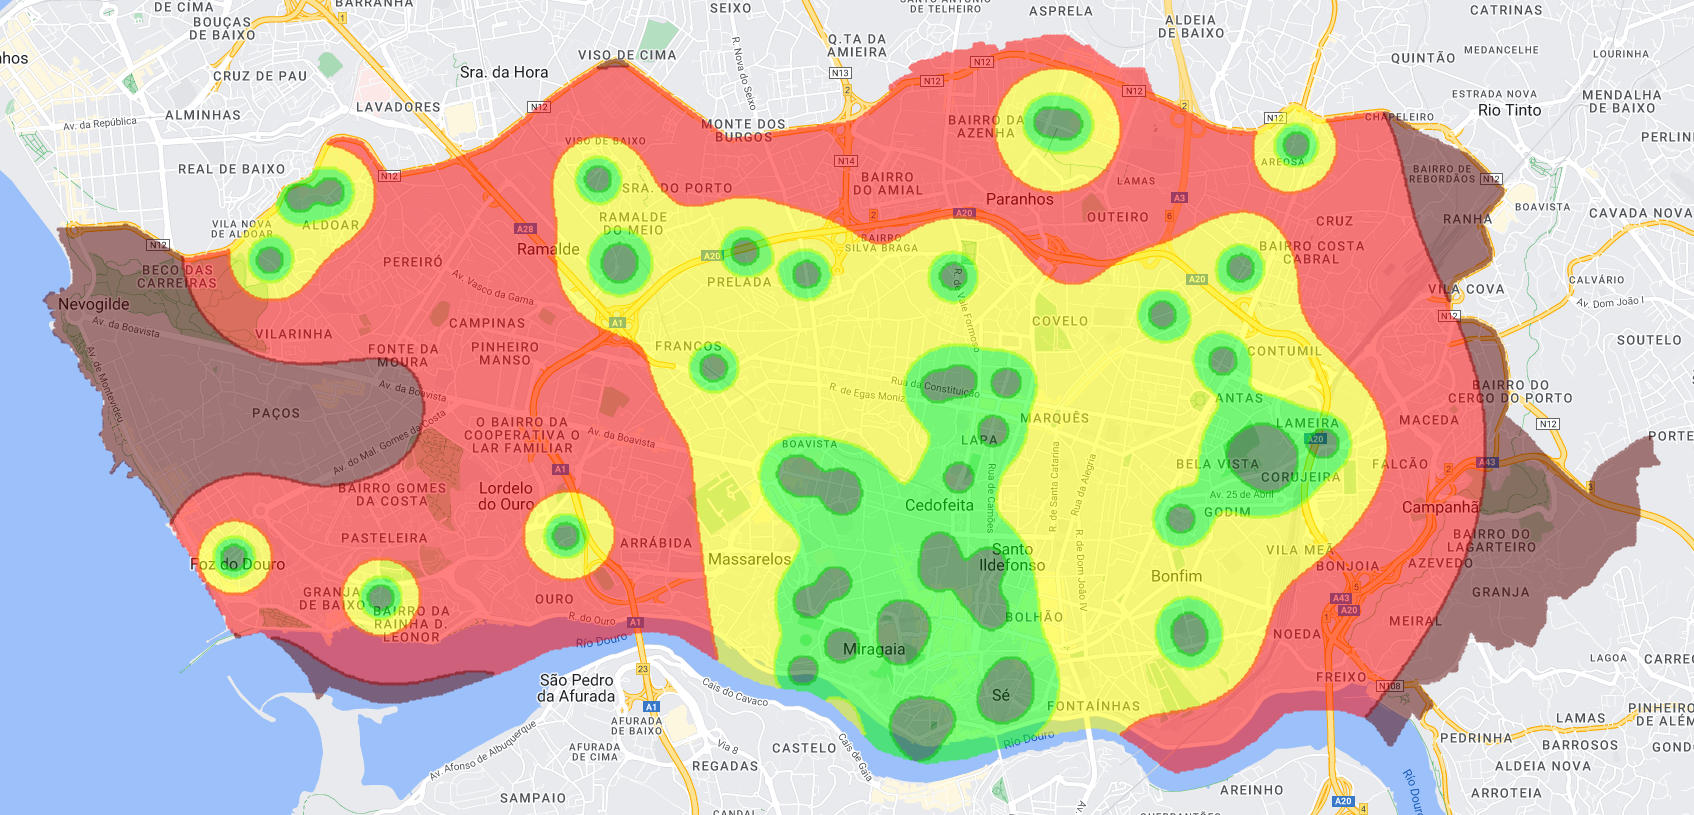
\includegraphics[width=0.9\linewidth]{Chapters/2-EDUs/images/porto_M5_no_weight.png}
    \caption{Computed zones for the city of Porto for five different mitigation levels, with dark-green representing the lowest risk while dark-red is the highest.}
    \label{Fig:zones_porto_5}
\end{figure}

It is interesting to notice that for higher values of $|M|$, the city is divided into more mitigation levels, but the practical outcome for sensors positioning may be not very different. Since we are using a natural logarithmic scale (Equation \ref{eq:risk_class}), the number of safer zones will be reduced, but the overall ``shape'' of adjacent mitigation zones will be almost the same, as we can see when comparing Figure \ref{Fig:zones_porto_3} and Figure \ref{Fig:zones_porto_5}. This way, after different tests for both Porto and Paris, with $|M|$ ranging from 2 to 10, we believe that $|M|=3$ may be a more usual configuration, defining three levels of criticality (bad, medium and good), which is very common in emergencies management systems \cite{surveyEmergencies}.

As an important remark, the adoption of a natural logarithmic scale in Equation \ref{eq:risk_class} creates a radial behaviour for sensors monitoring, usually irradiating from the cities' central areas where most emergencies-response facilities are located. We argue that this configuration for the mitigation zones may be more meaningful for EDUs positioning, but future works could adopt a scalar scale instead. Whatever the case, this could only change the computing of the mitigation levels, with no direct impact on the definitions of the proposed mathematical model and algorithms, leaving this choice for future evaluations.

Other set of experiments was concerned with the relevance weight of the points of interest. Figure \ref{Fig:zones_porto_3_weight} presents one of the results when $|M|=3$, assuming that $f(p)=10$ for hospitals, $f(p)=5$ for fire departments, $f(p)=2$ for police stations, and $f(p)=1$ for metro stations, considering that all PoIs of the same ``type'' have the same relevance weight. Since we have the definition of a MZ as $l = 10m$, we had 413,012 mitigation zones computed for the city of Porto.

%%%%%% Zonas para Porto, M = 3, PoI com diferentes weights
\begin{figure}[ht!]
    \centering
    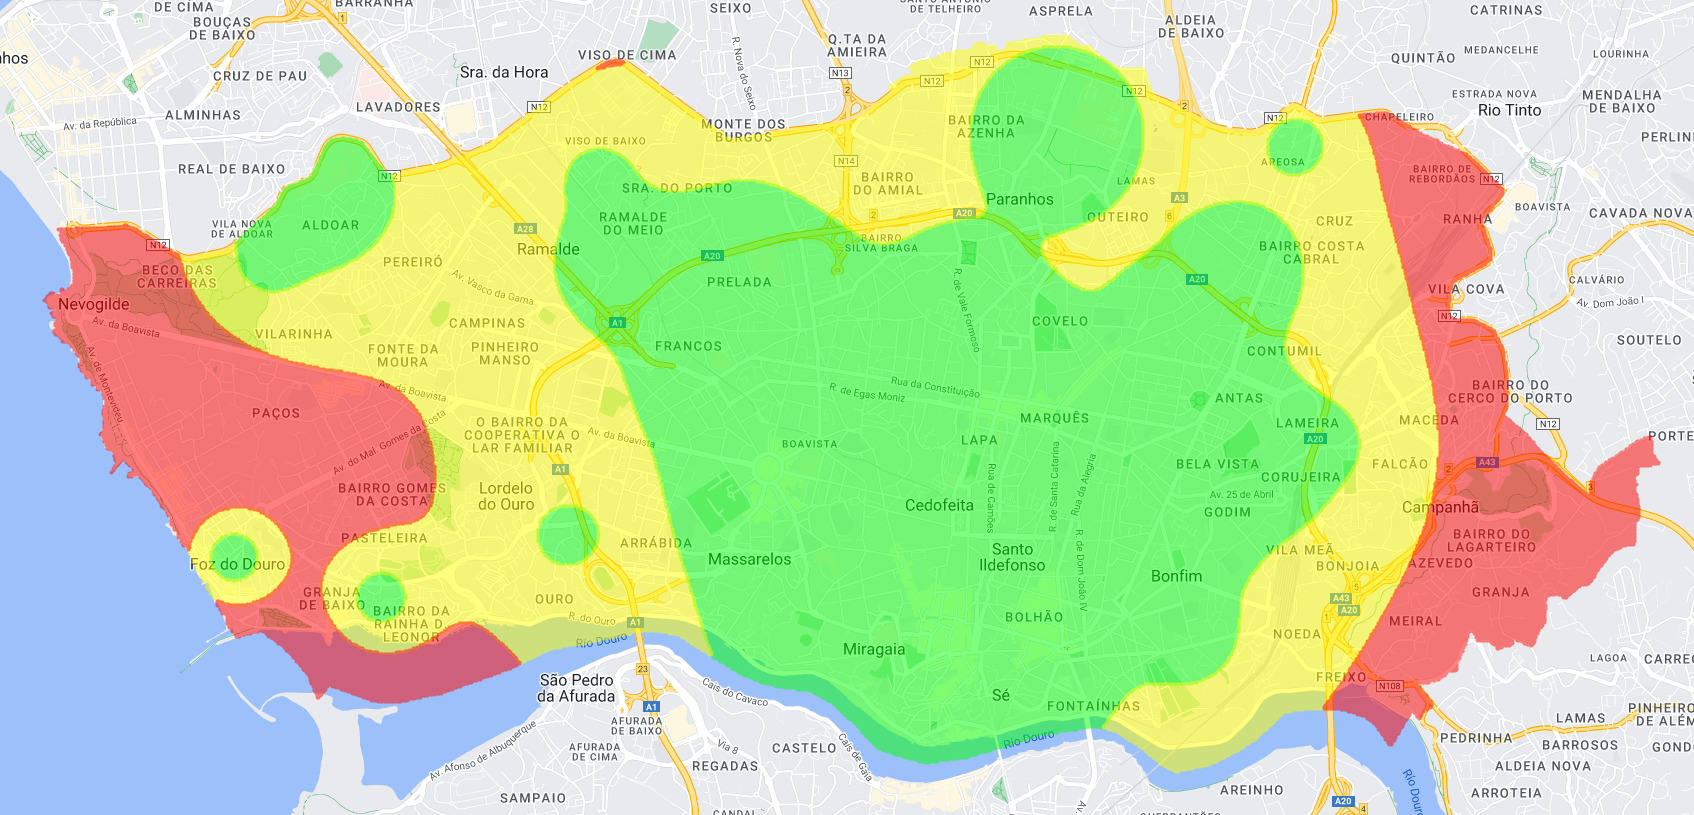
\includegraphics[width=0.9\linewidth]{Chapters/2-EDUs/images/porto_M3.png}
    \caption{Computed zones for the city of Porto, with $|M|=3$ and different relevance for the list of PoIs.}
    \label{Fig:zones_porto_3_weight}
\end{figure}

The weight of a PoI has the function to better set the relevance for mitigation responses in a city and thus this allows that the particularities of the selected urban area will be properly considered in the modelled scenario. Obviously, such settings will allow not only a differentiation of the types of response-related facilities, but also the configuration of a particular PoI relevance over others of the same type (e.g. when a particular hospital is bigger or better equipped than others). Doing so, the proposed approach assures a significant level of flexibility when modelling cities and emergencies management systems.

After all performed experiments, we achieved two different conclusions: first, considering practical adoption of mitigation zones in a city, $|M|=3$ seems to be the ideal configuration parameter to guide the positioning of EDUs; second, the relevance weights of the PoIs are more effective when there are some response centres that are notably much more relevant than others, once their actual positions seemed to play a more relevant role when computing mitigation zones than their relevance weights.  

%%%%%%%%%%%
\subsection{EDUs positioning}

After computing the mitigation zones for different parameters, the proposed EDUs positioning algorithms could be evaluated. For that, in order to create a uniform reference for comparison purposes, the mitigation zones created for the city of Porto when $|M|=3$ were considered, as depicted in Figure \ref{Fig:zones_porto_3_weight}. We assume the same weight configurations in that Figure, which is $f(p_h)=10$, $f(p_f)=5$, $f(p_p)=2$, and $f(p_m)=1$, for all $p_h \in P$ as hospitals, $p_f \in P$ as fire departments, $p_p \in P$ as police stations, and $p_m \in P$ as metro stations. Additionally, it is defined that $U=300$ for all experiments.

Figure~\ref{Fig:edus_random} presents the graphical results for the proposed Random algorithm.

\begin{figure}[htbp!]
    \centering
    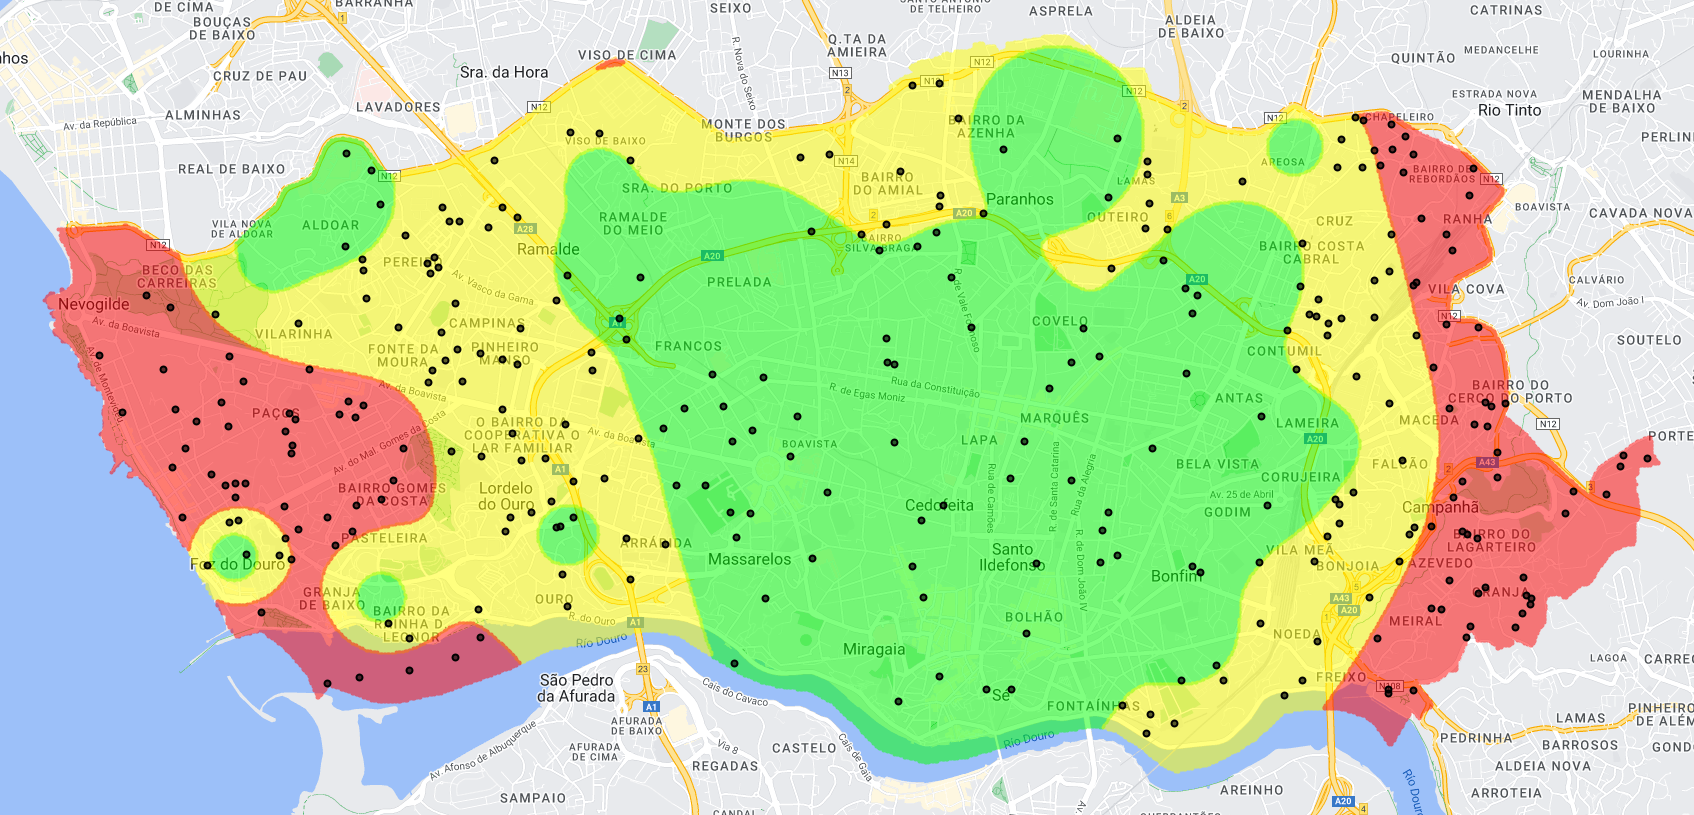
\includegraphics[width=0.9\linewidth]{Chapters/2-EDUs/images/porto_M3_random.png}
    \caption{Random positioning algorithm.}
    \label{Fig:edus_random}
\end{figure}

As expected, the randomly positioned EDUs do not have any specific criteria for positioning, leading to some undercovered areas and overlapping. In that Figure, the black spots are the suggested computed positions for deployment of the available EDUs.

In order to address most problems of the Random positioning approach, the Balanced algorithm was assessed in the same scenario, as presented in Figure~\ref{Fig:edus_balanced}.

\begin{figure}[htbp!]
    \centering
    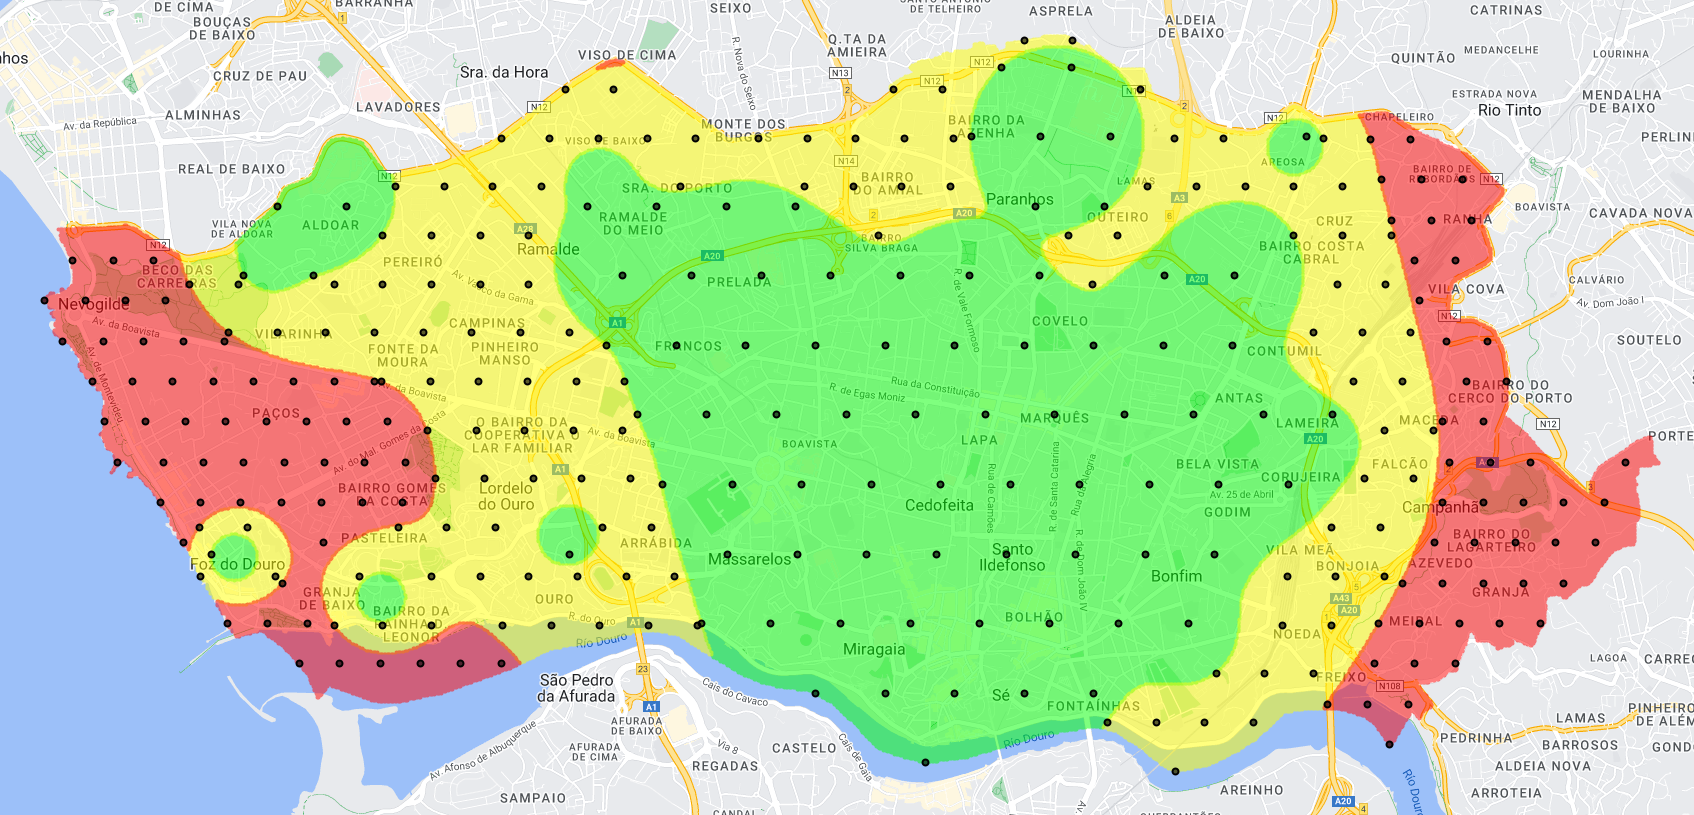
\includegraphics[width=0.9\linewidth]{Chapters/2-EDUs/images/porto_M3_balanced.png}
    \caption{Balanced positioning algorithm.}
    \label{Fig:edus_balanced}
\end{figure}

The Balanced algorithm performed better, but some EDUs were positioned very close to other units around the borders of the zones. Figure~\ref{Fig:edus_enhanced} presents the Balanced+ algorithm, which overcomes these drawbacks.

\begin{figure}[htbp!]
    \centering
    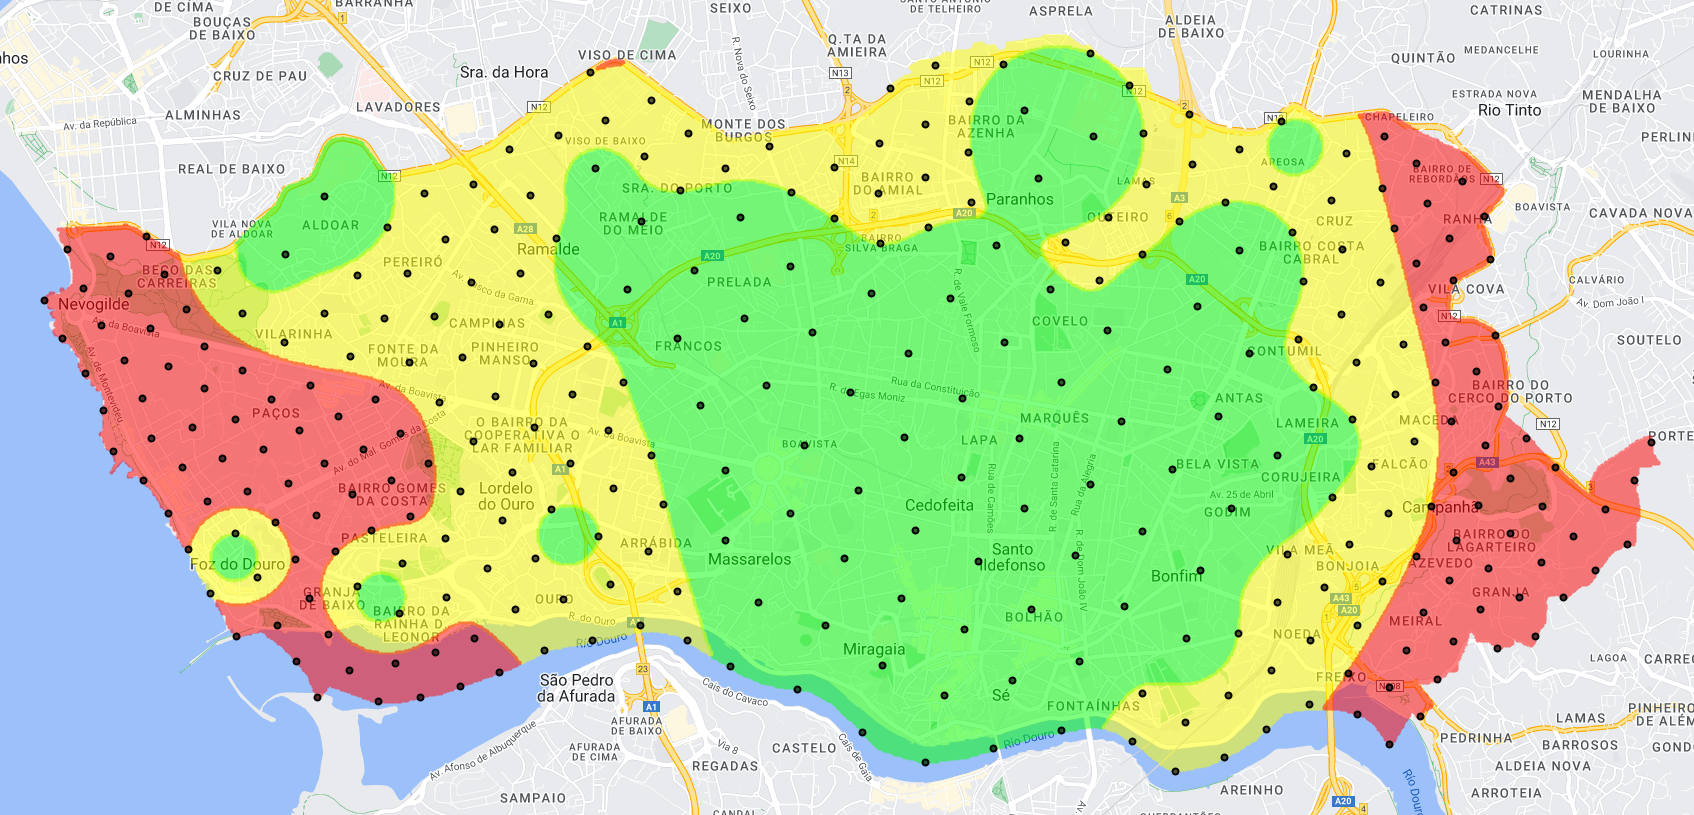
\includegraphics[width=0.9\linewidth]{Chapters/2-EDUs/images/porto_M3_balanced_plus.png}
    \caption{Balanced+ positioning algorithm.}
    \label{Fig:edus_enhanced}
\end{figure}

Finally, Figure~\ref{Fig:edus_restricted} presents the results for the Restricted algorithm, which we expect to have the most realistic outcome. Now, the EDUs are only positioned on allowed spots, for example avoiding that EDUs are positioned over the water as it may happen in the other algorithms.  

\begin{figure}[htbp!]
    \centering
    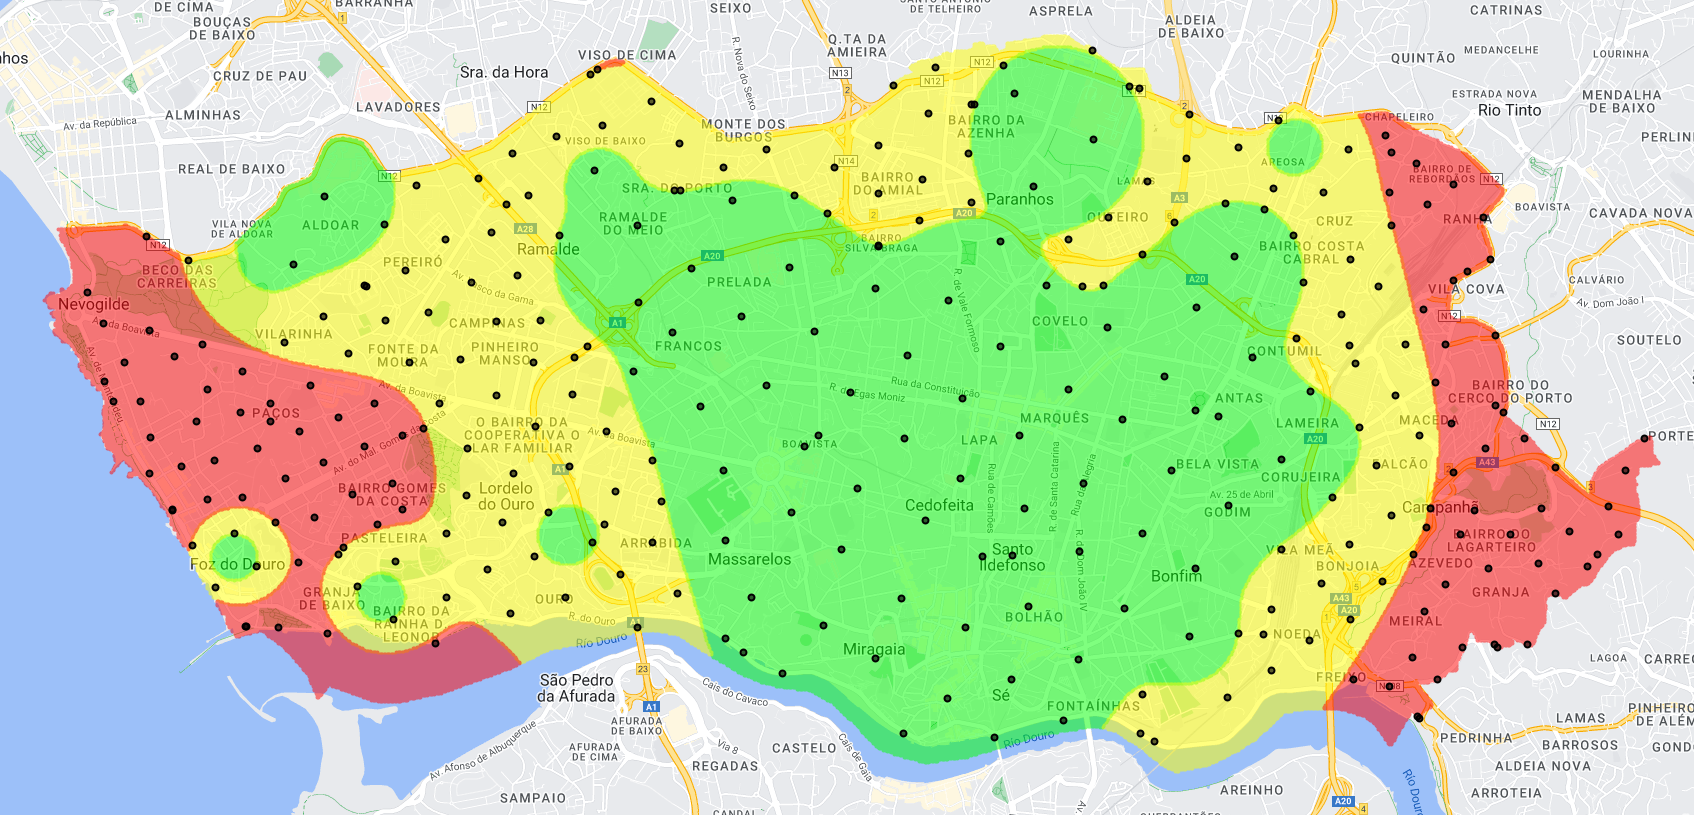
\includegraphics[width=0.9\linewidth]{Chapters/2-EDUs/images/porto_M3_restricted.png}
    \caption{Restricted positioning algorithm.}
    \label{Fig:edus_restricted}
\end{figure}

When comparing the different results for the Balanced+ and the Restricted algorithms, it is possible to note that the positions of the EDUs are almost the same, varying in just a few meters according to the existence of roads (more realistic spots for deployment of the units). However, such small difference achieves a more realistic result, which should be considered for actual deployment in most cases.

%%%%%%%%%
\subsection{Practical issues and performance evaluations}

When analysing the achieved experimental results with real data from two different large cities, it is possible to see that more critical areas concerning mitigation response will receive more sensors than less critical areas, which may reduce the time between effective detection and response to emergencies. Actually, this is an average reasoning about how emergencies management systems can be deployed, but it already opens new possibilities when planning such systems. Since the proposed mathematical model fits to the particularities of any city, and real OpenStreetMap data is processed as input, the proposed approach as a whole could be applied to any city in the world, which is in fact one of the major goals of this work. The performed evaluations for two different cities concerning both size and urban infrastructure are important demonstrations of the applicability of the proposed approach, which can consider not only any city as input, but also different configuration parameters.

When applying the proposed approach, the size of the AoI, the width/height of mitigation zones and the number of possible mitigation levels are not only important configuration parameters that deals with accuracy, but they will also be related to the computational costs to process the algorithms. However, it is expected that the computation of mitigation levels will be performed only once, typically just after changes in the number and configurations of the list of PoIs. In fact, after computation of the mitigation zones, the chosen positioning algorithm may be executed as a response to a new number of available EDUs, achieving new configurations and helping when searching for the ideal number of EDUs for deployment in a city. 

In order to demonstrate the computational costs of the algorithms, the execution time for the experiments on an AMD Ryzen 5 4600h processor with 16 GB RAM computer was accounted. The execution time of the algorithms for both Porto ($|M|=3$ and $U=300$) and Paris ($|M|=3$ and $U=600$) are presented in Table \ref{Table:costs}.

\begin{table}
    \centering
    \caption{Execution time in seconds for the positioning algorithms.}
    \label{Table:costs}
    \begin{tabular}{|c|c|c|}
        \hline
        \textbf{Algorithm} & \textbf{Porto} & \textbf{Paris} \\
        \hline
        Random  &  0.124 &  0.215 \\ 
        \hline
        Balanced  & 5.692  &  10.974 \\ 
        \hline
        Balanced+  & 107.578 &  316.359  \\ 
        \hline
        Restricted  & 108.716  & 325.006 \\ 
        \hline
    \end{tabular}
\end{table}

The execution time of the positioning algorithms will increase for more complex algorithms, but they will usually deliver better results. In fact, the execution of the positioning algorithms is not the most time-demanding part of the proposed approach, with most time being spent to compute the mitigation zones. For example, when having $|M|=3$, Porto (Figure \ref{Fig:zones_porto_3_weight}) took 998.46 seconds while Paris (Figure \ref{Fig:zones_paris_3}) needed 1341.99 seconds to compute all mitigation zones. At this point, as expected, we can conclude that the final computational cost will depend on multiple variables, although the processing time is not a critical situation in this problem scope.

Finally, the employed geospatial data source could be considered as an important parameter when adopting the proposed approach, affecting the overall processing time of the algorithms. Although the proposed approach is not dependent on the OpenStreetMap database, it is assumed as the reference for processing of mitigation zones, mostly due to the fact that it is an open geospatial database that is collaboratively managed and updated. As long as it is regarded as a reliable source of data to compute mitigation zones, the time needed to pre-process a city and select all PoIs was not significant when using OSM, since such list (and related metadata) was processed in few seconds. However, when other sources of data are selected, the data acquisition time and general data reliability may be important issues that have to be properly considered.

%%%%%%%%%%%%%%%%%%%%%%%%%%%%%5
\section{Discussions and perspectives}
\label{S:6}

As discussed throughout this article, the positioning of the EDUs in a city is a very important issue for emergencies detection units, which reinforces the need for flexible positioning algorithms. Overall, the detection of emergencies in smart cities is the first step when handling critical situations in urban areas, and thus the proposed approach comes as a valuable pre-deployment step in such scenario. In this article, we argue that distributed sensors will be one of the main data sources when detecting emergencies, which put their proper assembling, programming, positioning, and deployment, as major issues to be improved. At this point, while the construction of emergencies detection units have been addressed lately \cite{hardware1,hardware2}, their positioning in a city still has many challenges when emergencies detection is being performed.

The four proposed algorithms presented valuable results to guide the deployment of EDUs in a city, mainly when taking the more realistic Balanced+ and Restricted algorithms. As discussed before, this is accomplished by exploiting geospatial data of emergency-response urban infrastructure, which allows the computation of real positions for the units. However, the actual deployment of the units and the issues associated to it such as physical attachment, energy supply, networking coverage, transmission throughput, among others, are out of the scope of this work since they are more related to wireless sensor networks and Internet of Things (IoT) systems than smart cities planning. Additionally, actual deployment of the EDUs would not be very significant to evaluate the proposed algorithms themselves, but it could be valuable when pursing other research goals than the ones already addressed in this work. Finally, due to the necessary cost to deploy hundreds or thousands of EDUs in a city just to evaluate the proposed algorithms, additional evaluations with physical units were not performed.

Still considering additional research issues for actual deployment, it is reasonable to expect that the EDUs will be usually deployed on the outdoors, potentially in public areas. For such deployment, EDUs could be attached to trees, electric poles, bus stops, traffic lights, among other spots. Moreover, public buildings such as schools, post offices and even the city hall could be adopted as deployment spots once they are very close to the area suggested by the proposed algorithms, facilitating actual deployment. 

Other important remark is that some networking issues such as connectivity, throughput, availability, and even security, were not considered by the proposed positioning algorithms, which might lead to disconnected EDUs in cities with poor networking infrastructures. Actually, we consider that these networking ``parameters'' should be processed in a post-positioning phase of the proposed approach, potentially supporting a fine-grained positioning of the EDUs. This way, networking would behave like a response layer, but it would not be directly used to define positioning zones. The idea would be to perform small reallocations of the EDUs within the same mitigation zones when some defined networking quality parameter is improved. In fact, we believe that networking could be incorporated to the proposed solutions through a mathematical model when the actual networking infrastructure of a city is properly known. This remark will be considered in future works.

Finally, after the performed experiments have given important clues about the practical effectiveness of the proposed approach, we could wonder about the way cities may be perceived when mitigating emergencies. Actually, the definition of mitigation zones might be perceived as a Response Layer in a more generic term, which would be only one step of a more comprehensive solution when guiding the positioning of EDUs. Doing so, for example, the average traffic accidents in an urban area could also be defined as a response layer, which would be applied after or before the processing of the mitigation response layer. And the same could be done when accounting the presence of dangerous facilities, such as a factory of dangerous chemical products, or even a nuclear station. In this same direction, the relief of a city could also be processed as a layer that could complement the 2D perspective of zones adopted in this work, for example allowing the processing of higher (or lower) areas as more/less critical for emergencies. Whatever the case, all of these conceptual layers can be processed sequentially in a balanced way, resulting in an integrated perception of risks that will ultimately result in a combined risk index for each subarea in a city. Nevertheless, although we believe that such multi-layers perception is promising, we expect that future solutions can be applied mathematically in a generic way, exploiting open geospatial data from open databases.


%%%%%%%%%%%%%%%%%%%%%%%%%%%%%5
\section{Conclusions}

This article proposed a comprehensive mathematical model and four different positioning algorithms to guide the deployment of Emergencies Detection Units in a city. For that, the concept of mitigation zone was proposed and the procedures to exploit it to position EDUs in a more efficient way were discussed. With the performed experiments, practical issues were analysed, as well as the computational costs of the solutions were accounted. At the end, the expected results of this work were achieved. 

In general, resilience to detected emergencies has been a recurrent issue when creating smart cities. At this sense, although only part of the overall emergencies management cycle was addressed in this article, EDUs positioning has not been properly considered as an actual problem for macro-system solutions that consider an entire city as a deployment area. Therefore, the proposed approach comes as an important improvement to this research area, potentially fostering new investigation efforts in the positioning and deployment of multi-sensor units in smart cities.

As discussed in the previous section, future works will be concerned with the evaluation of the proposed model in order to consider other geospatial urban data, complementing the existence of mitigation response centres. Moreover, other positioning algorithms will be proposed and evaluated, trying to better optimise the positioning of the EDUs. Finally, genetic algorithms will be considered to compute the positions of the EDUs when input parameters other than mitigation zones are considered, opening a new research trend in this area.

% \section{Acknowledgement}

% This work is financially supported by national funds through the FCT/MCTES (PIDDAC), under the project EXPL/EEI-COM/1089/2021. It is also supported by INEGI-LAETA (FCT project UIDB/50022/2020). Finally, this work was financed in part by the Coordenação de Aperfeiçoamento de Pessoal de Nível Superior - Brasil (CAPES) - Finance Code 001.

\printbibliography[heading=subbibliography]

\end{refsection}
